
{ \setbeamercolor{background canvas}{bg=hl_bg}
  \setbeamercolor{normal text}{fg=hl_fg}
  \setbeamercolor{frametitle}{fg=hl_fg}
  \begin{frame}
    \usebeamercolor[fg]{normal text}
    \begin{center}
      {
        \begin{tikzpicture}
          \tikzstyle{cnode} = [thick, draw=white, ellipse, inner sep = 2pt,  align=center]
          \tikzstyle{fnode} = [thick, draw=white, ellipse, inner sep = 10pt,  align=center]
          \tikzstyle{rnode} = [thick, rectangle, inner sep = 1.5pt,  align=left]
          \node[rnode] (inf) at (-2, 0) {\large Inference};
          \node[rnode, below = 0.6cm of inf.west, anchor=west] (abp) {$\bullet$ {$\alpha$-BP}};
          \node[rnode, below = 1.2cm of inf.west, anchor=west] (renn) {$\bullet$ RENN};
          \node[cnode, fit=(abp)(inf)(renn)] (infn) {};
          
          \node[rnode, right = 3 of inf] (lern) {\large Learning};
          \node[rnode, below = 0.4 of lern.west, anchor=west] (genmm) {\textbf{$\bullet$ GenMM}};
          \node[rnode, below = 0.8 of lern.west, anchor=west] (genhmm) {\textbf{{$\bullet$} GenHMM}};
          \node[rnode, below = 1.2 of lern.west, anchor=west] (lfree) {{$\bullet$} EOTGM};
          \node[cnode, fit=(lern)(genmm)(genhmm)(lfree)] (learn) {};
          \node[rnode, draw=green, fit=(genmm)(genhmm)] () {};

          \node[fnode, fit=(infn)(lern)] (box) {};

          
          \node[below right = 0.5 and -0.5 of infn] {{Probabilistic} Graphical Model};
          \draw[->,line width=0.2mm] (infn) to[out=15, in=165] (learn);
          \draw[->,line width=0.2mm] (learn) to[out=195, in=-15] (infn);
        \end{tikzpicture}
      }
    \end{center}
    
  \end{frame}
}
\begin{frame}[label=current]
  {Incomplete Observation}
  Partial observation: $\bm{x} = [  \underbrace{\bm{x}_U}_{Unobserved}, \underbrace{\bm{x}_O}_{Observed}]$
  \begin{equation*}
    l(\bm{x}_O; \bm{\theta}) = \log{\sum_{\bm{x}_U}p(\bm{x}_U, \bm{x}_O; \bm{\theta})} = \log{\underbrace{Z(\bm{x}_O;\bm{\theta})}_{\sum_{\bm{x}_U}\tilde{p}(\bm{x}; \bm{\theta})}} - \log{Z(\bm{\theta})},
  \end{equation*}

  {Connect Free Energy to Evidence Lower Bounder}:
  \begin{columns}
    \column{0.6\textwidth}
    \begin{align*}
      l(\bm{x}_O; \bm{\theta}) &\geq - \underbrace{F_v(q(\bm{x}_U|\bm{x}_O))}_{Variational Free Energy} - \log{Z(\bm{\theta})} \nonumber \\
                               & = \EE_{q(\bm{x}_U|\bm{x}_O)}\left[ \log{\frac{{p}(\bm{x}_U, \bm{x}_O; \bm{\theta})}{q(\bm{x}_U|\bm{x}_O)}} \right] \nonumber \\
                               & = \underbrace{\EE_{q(\bm{x}_U|\bm{x}_O)}\left[ \log{{p}(\bm{x}_U, \bm{x}_O; \bm{\theta})} \right] + H({q(\bm{x}_U|\bm{x}_O)})}_{\text{Evidence Lower Bound $F(q, \bm{\theta})$}}
    \end{align*}
    
    \column{0.4\textwidth}
    Intuition of maximizing $F(q,\bm{\theta})$
    \begin{itemize}[label=\textbullet]
    \item Maximizing (incomplete) likelihood
    \item Minimizing free energy
    \end{itemize}

  \end{columns}
  This gives the EM as a coordinate ascent method:
  \begin{align*}
    \mathrm{E~step:}~~~ q^{(t+1)} &= \uargmax{q}{F(q, \bm{\theta}^{(t)})}, \\
    \mathrm{M~step:}~~~\bm{\theta}^{(t+1)} &= \uargmax{\bm{\theta}}{F(q^{(t+1)}, \bm{\theta})}.
  \end{align*}
\end{frame}


\begin{frame}[label=current]{Generator Mixed Model}
  {Equipping EM with Normalizing Flows}
  \begin{columns}
    \column{0.4\textwidth}
    \centering
    \begin{tikzpicture}
      \tikzstyle{enode} = [thick, draw=black, circle, align=center]
      \tikzstyle{cnode} = [thick, draw=black, circle, align=center, inner sep = 0.3pt]
      \tikzstyle{nnode} = [thick, rectangle, rounded corners = 2pt,minimum size = 0.8cm,draw,inner sep = 12pt]
      %%%%%%%%%%%%%%%%%%%%%%%%%%%%%%%%%%%%%%%% 
      %% directed graphical model
      %%%%%%%%%%%%%%%%%%%%%%%%%%%%%%%%%%%%%%%% 
      \begin{scope}[scale=1, every node/.append style={transform shape}]
        \node[enode] (x) at (0,0){$\bm{x}$};

\node[enode, above=of x] (s) {$\bm{s}$};
\node[enode, left=of s] (z) {$\bm{z}$};
\node[enode, right=of s] (pi) {$\bm{\pi}$};
\node[cnode, right=of x] (phi) {$\{ \bm{\theta}_k \}$};
\node[nnode, fit=(x)(z)(s)] (box) {};

\draw[->] (z) to (x);
\draw[->] (s) to (x);
\draw[->] (pi) to (s);
\draw[->] (phi) to (x);

%%% Local Variables:
%%% mode: latex
%%% TeX-master: "../ppgm_slide"
%%% End:

      \end{scope}

    \end{tikzpicture}
    
    \column{0.55\textwidth}
    
    \centering
    \begin{minipage}{\linewidth}
      
      \begin{itemize}[label=\textbullet]
      \item Ideal case: The underline true $p^{\ast}(\bm{x})$ is in hypothesis space $\Hh$, i.e. $p^{\ast}(\bm{x}) \in \Hh$.
      \item Out of reach: Test $p^{\ast}(\bm{x}) \stackrel{?}{\in} \Hh$
      \item A general desire:
        \begin{equation*}
          \Hh ~\mathrm{is~large}  \rightarrow \mathrm{condidate}~ p(\bm{x};\bm{\theta})~\mathrm{is~flexible}
        \end{equation*}
        
      \end{itemize}
      
      This brings up the finite \textbf{mixture} models.

      \begin{align*}\label{eq:FirstMixtureModel}
        p(\bm{x};\bm{\Theta})  = \textstyle\sum_{k=1}^K \pi_k  p_k(\bm{x}) = \textstyle \sum_{k=1}^K \pi_k  p(\underbrace{\bm{g}(\bm{z};\bm{\theta}_k)}_{\text{\begin{tabular}{c}Variable change \\via generator $\bm{g}$\end{tabular}}}).
      \end{align*}
      
    \end{minipage}
  \end{columns}
  
  \vskip -0.5cm
  What to expect from GenMM:
  \begin{itemize}[label=\textbullet]
  \item {Flexible and expressive model, enlarging hyperspace $\Hh$}
  \item {Tractable likelihood} 
  \item {Compatible with typical statistical models}
  \item Compatible with NN tools/frameworks
  \item {Scale to high-dimensional structured data}
  \item {Efficient in sampling (data generation)}
  \item {...}
  \end{itemize}

\end{frame}




\begin{frame}[label=current]{A High-level View of GenMM: finite mixture}
  \begin{tikzpicture}
    \tikzstyle{enode} = [thick, draw=black, circle, align=center]
    \tikzstyle{cnode} = [thick, draw=black, circle, align=center, inner sep = 0.3pt]
    \tikzstyle{nnode} = [thick, rectangle, rounded corners = 2pt,minimum size = 0.8cm,draw,inner sep = 22pt]
    %%%%%%%%%%%%%%%%%%%%%%%%%%%%%%%%%%%%%%%% 
    %% 1. directed graphical model
    %%%%%%%%%%%%%%%%%%%%%%%%%%%%%%%%%%%%%%%% 
    \begin{scope}[scale=0.6, every node/.append style={transform shape}, local bounding box=dgm, opacity=0.3]
      \node[enode] (x) at (0,0){$\bm{x}$};

\node[enode, above=of x] (s) {$\bm{s}$};
\node[enode, left=of s] (z) {$\bm{z}$};
\node[enode, right=of s] (pi) {$\bm{\pi}$};
\node[cnode, right=of x] (phi) {$\{ \bm{\theta}_k \}$};
\node[nnode, fit=(x)(z)(s)] (box) {};

\draw[->] (z) to (x);
\draw[->] (s) to (x);
\draw[->] (pi) to (s);
\draw[->] (phi) to (x);

%%% Local Variables:
%%% mode: latex
%%% TeX-master: "../ppgm_slide"
%%% End:

    \end{scope}
    
    %%%%%%%%%%%%%%%%%%%%%%%%%%%%%%%%%%%%%%%% 
    %% 2. illustration of GenMM
    %%%%%%%%%%%%%%%%%%%%%%%%%%%%%%%%%%%%%%%% 
    \begin{scope}[shift={($(dgm.east)+(3cm,0)$)}, local bounding box=illsGenMM]
      
% \tikzstyle{enode} = [thick, draw=blue, circle, inner sep = 3pt,
% align=center]
\tikzstyle{enode} = [thick, draw=black, ellipse, inner sep = 2pt,  align=center]
\tikzstyle{nnode} = [thick, rectangle, rounded corners = 2pt,minimum size = 0.8cm,draw,inner sep = 2pt]
\node[enode,label={below:{\tiny Shared latent source}}] (z) at (0,0) {$\bm{z}\sim p(\bm{z})$};
\node[enode, label={below:{\tiny Induced distribution}}] (x) at (5.5,0){$\bm{x}\sim p(\bm{x}; \bm{\Phi})$};
% \node at (5.2,-1) {$p(\bm{x};\bm{\Phi}) = \textstyle\sum_{k=1}^K \pi_k  p_k(\bm{x})$};
\node[nnode] (g1) at (2.6,1.8) {$\bm{g}_1$};
\node[nnode] (g2) at (2.6,0.5) {$\bm{g}_2$};
\node[nnode] (gk) at (2.6,-1.8) {$\bm{g}_K$};
\draw[dotted,line width=2pt] (2.6,-0.3) -- (2.6,-1.2);
\draw[->] (z) [in= 180, out =0] to (g1);
\draw[->] (z) [in= 180, out =0] to (g2);
\draw[->] (z) [in= 180, out =0] to (gk);
\filldraw[->] (3.7, 0.5)circle (2pt) -- node[above=0.2](switch){$\bm{s}\sim \bm{\pi}$} (x);
\node[above= 0.2 of switch.east] {\tiny \begin{tabular}{c}Categorical variable\\ as generator switch\end{tabular}};
% \draw[->] (3,-0.8) -- (3.5, -0.8);
\draw[->] (g1) -- (3.5,1.8);
\draw[->] (g2) -- (3.5, 0.5);
\draw[->] (gk) -- (3.5, -1.8);
\begin{scope}[on background layer, every node/.append style={transform shape}]
\node [rounded corners = 2pt, inner sep=4pt, fill=blue!30,fit=(g1)(g2)(gk), label={[label distance=0.3cm]-60:{\tiny Mixture of generators}}] {};
\end{scope}
%%% Local Variables:
%%% mode: latex
%%% TeX-master: "../ppgm_slide"
%%% End:

    \end{scope}
    \draw[green, ->, shorten >=5pt, shorten <=5pt] (dgm) --node [text width=2cm, black, midway,above]{\tiny Alternative illustration of GenMM} (illsGenMM);
    
    %%%%%%%%%%%%%%%%%%%%%%%%%%%%%%%%%%%%%%%% 
    %% 3. illustration of flow
    %%%%%%%%%%%%%%%%%%%%%%%%%%%%%%%%%%%%%%%% 

    \begin{scope}[shift={($(illsGenMM.south)+(-1cm,-1cm)$)}, scale=0.8, local bounding box=illFlow,opacity=\bgopacity]
      \def\layersep{1.5cm}
\begin{scope}[shorten >=1pt,->,draw=black!50, node distance=\layersep, scale=0.6, every node/.append style={transform shape},transform shape, local bounding box=ffnn]
  \tikzstyle{every pin edge}=[<-,shorten <=1pt]
  \tikzstyle{neuron}=[circle,fill=black!50,minimum size=17pt,inner sep=0pt]
  \tikzstyle{input neuron}=[neuron, fill=green!80];
  \tikzstyle{output neuron}=[neuron, fill=red!80];
  \tikzstyle{hidden neuron}=[neuron, fill=blue!80];
  \tikzstyle{annot} = [text width=4em, text centered]

  % Draw the input layer nodes
  \foreach \name / \y in {1,...,4}
  % This is the same as writing \foreach \name / \y in {1/1,2/2,3/3,4/4}
  % \node[input neuron, pin=left:Input \#\y] (I-\name) at (0,-\y) {};
  \node[input neuron, pin=left:{}] (I-\name) at (0,-\y) {};


  % Draw the hidden layer nodes
  \foreach \name / \y in {1,...,4}
  \path[yshift=0.0cm] node[hidden neuron] (H-\name) at (\layersep,-\y cm) {};

  % Draw the output layer node
  \foreach \name / \y in {1,...,4}
  \node[output neuron,pin={[pin edge={->}]right:{}}] (O-\name) at (2*\layersep, -\y cm) {};

  % Connect every node in the input layer with every node in the
  % hidden layer.
  \foreach \source in {1,...,4}
  \foreach \dest in {1,...,4}
  \draw[-{Stealth[scale=0.5]}] (I-\source) edge (H-\dest);

  % Connect every node in the hidden layer with the output layer
  \foreach \source in {1,...,4}
  \foreach \dest in {1,...,4}
  \draw[-{Stealth[scale=0.5]}] (H-\source) edge (O-\dest);

  % \foreach \source in {1,...,4}
  % \path (H-\source) edge (O);

  % Annotate the layers
  % \node[annot,above of=H-1, node distance=1cm] (hl) {Hidden layer};
  % \node[annot,left of=hl] {Input layer};
  % \node[annot,right of=hl] {Output layer};
  \node[inner sep=0pt, left= 0.2cm of ffnn] (latentz) {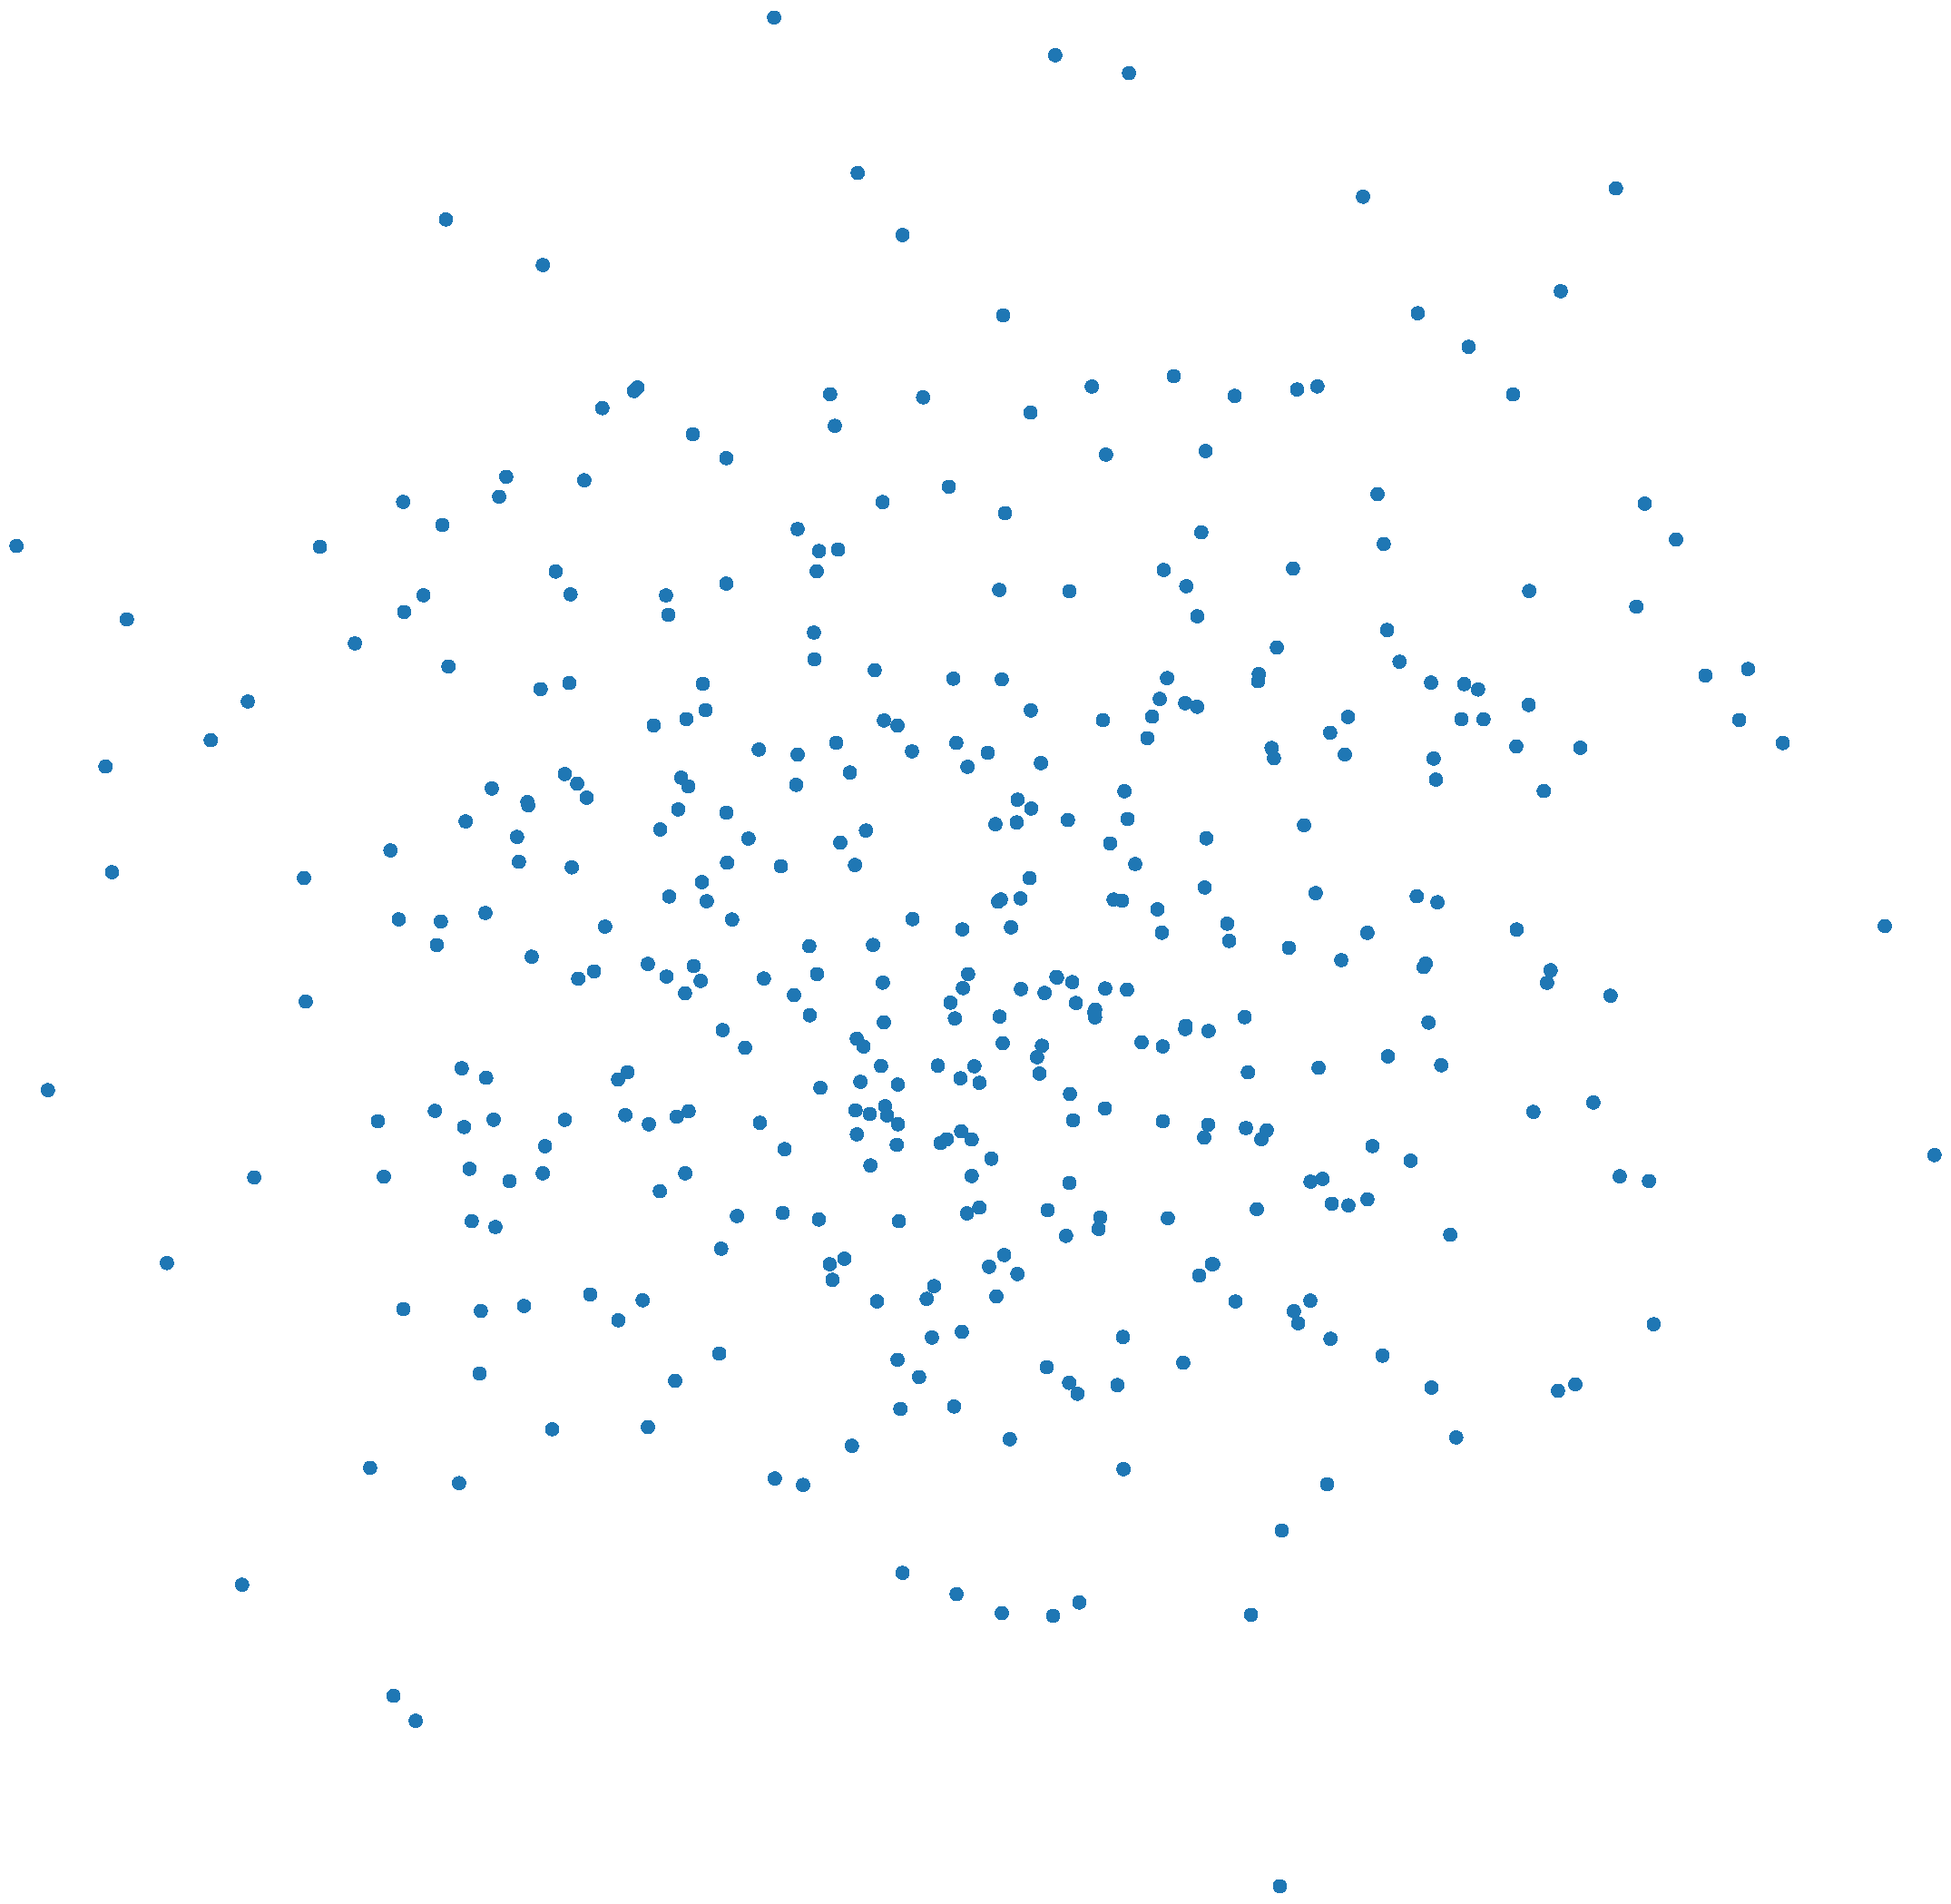
\includegraphics[width=.3\textwidth]{images/moon/zdist-crop.pdf}};
  \node[inner sep=0pt, right= 0.2cm of ffnn] (latentx) {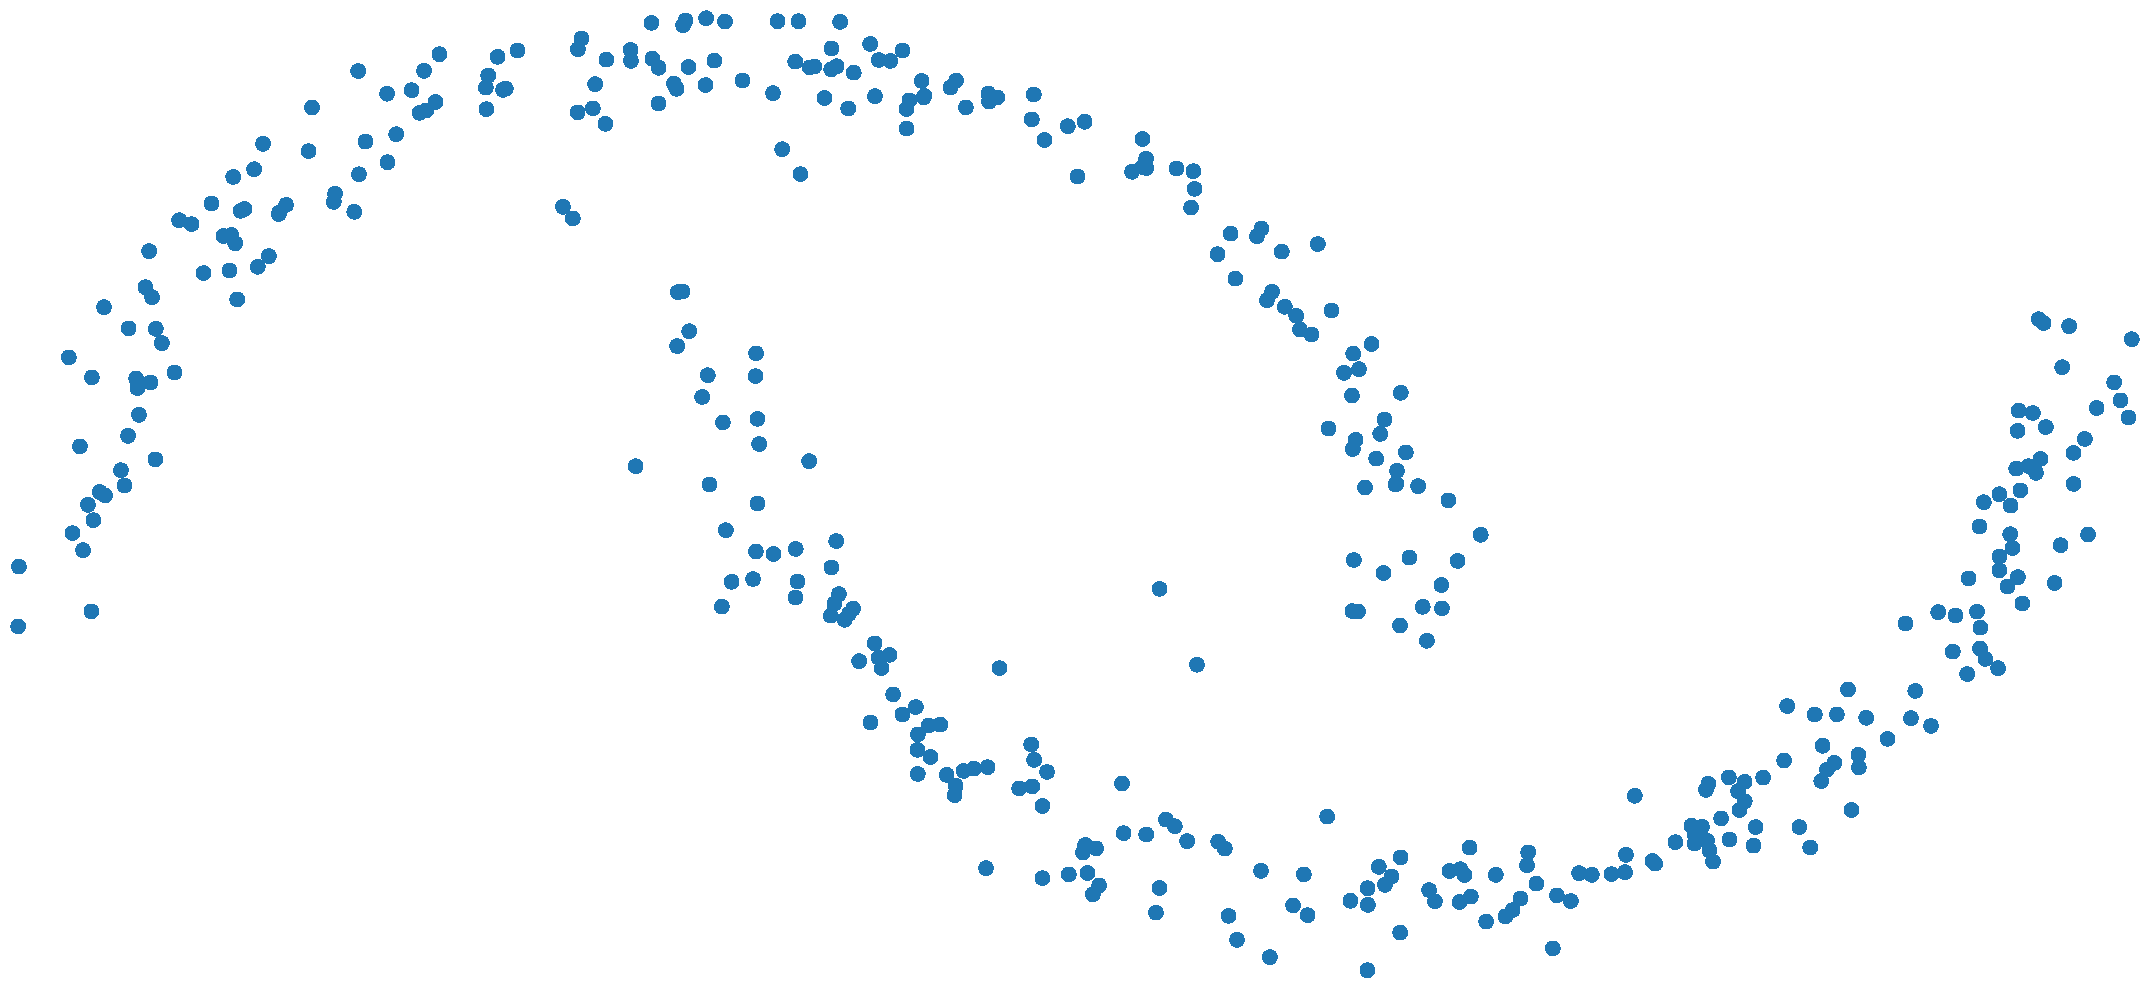
\includegraphics[width=.3\textwidth]{images/moon/xdist-crop.pdf}};
  
\end{scope}
%%% Local Variables:
%%% mode: latex
%%% TeX-master: "../ppgm_slide"
%%% End:

    \end{scope}
    
    \draw[dashed, ->, shorten >=5pt, shorten <=5pt, opacity=\bgopacity] ($(gk.north)+(0,-1.0cm)$) -- ($(gk.north)+(0,-2.0cm)$);
    
    %%%%%%%%%%%%%%%%%%%%%%%%%%%%%%%%%%%%%%%% 
    %% 4. one layer mapping of the flow
    %%%%%%%%%%%%%%%%%%%%%%%%%%%%%%%%%%%%%%%% 
    \draw[dashed, ->, shorten >=5pt, shorten <=5pt, opacity=\bgopacity] ($(latentz.west)+(-0.1cm,0)$) -- ($(latentz.west)+(-1.5cm,0)$);
    
    \begin{scope}[shift={($(dgm.south)+(0,-3.5cm)$)}, scale=0.5, every node/.append style={transform shape}, local bounding box=oneLayer, opacity=\bgopacity]
      % \tikzstyle{enode} = [thick, draw=blue, circle, inner sep = 3pt,
% align=center]
\tikzstyle{enode} = [thick, draw=black, circle, inner sep = 0, minimum size = 1cm,  align=center]
\tikzstyle{nnode} = [thick, rectangle, rounded corners = 2pt,minimum size = 0.4cm,draw,inner sep = 2pt]
\node[enode] (hal) at (-2,1) {$\bm{h}_{l,a}$};
\node[enode] (hbl) at (-2,-1) {$\bm{h}_{l,b}$};
\node[enode] (hal-1) at (2,1) {$\bm{h}_{l-1,a}$};
\node[enode] (hbl-1) at (2,-1) {$\bm{h}_{l-1,b}$};
\node[nnode] (times) at (-0.5,-1) {$\times$};
\node[nnode] (plus) at (0.5,-1) {$+$};
\node[nnode] (eq) at (0,1) {$=$};
\draw[->] (hal) -- node[fill=white] {$m_a$} (times);
\draw[->] (hal) -- node[fill=white] {$m_b$} (plus);
\draw[->] (hal) to (eq);

\draw[->] (eq) to (hal-1);
\draw[->] (hbl) to (times);
\draw[->] (times) to (plus);
\draw[->] (plus) to (hbl-1);
% \draw[draw=black] (-0.5,-0.5) rectangle ++(1,2);

%%% Local Variables:
%%% mode: latex
%%% TeX-master: "../ppgm_slide"
%%% End:

    \end{scope}
    
  \end{tikzpicture}
\end{frame}


\begin{frame}[label=current]{A High-level View of GenMM: flow gears}
  \begin{tikzpicture}
    \tikzstyle{enode} = [thick, draw=black, circle, align=center]
    \tikzstyle{cnode} = [thick, draw=black, circle, align=center, inner sep = 0.3pt]
    \tikzstyle{nnode} = [thick, rectangle, rounded corners = 2pt,minimum size = 0.8cm,draw,inner sep = 22pt]
    %%%%%%%%%%%%%%%%%%%%%%%%%%%%%%%%%%%%%%%% 
    %% 1. directed graphical model
    %%%%%%%%%%%%%%%%%%%%%%%%%%%%%%%%%%%%%%%% 
    \begin{scope}[scale=0.4, every node/.append style={transform shape}, local bounding box=dgm, opacity=0.3]
      \node[enode] (x) at (0,0){$\bm{x}$};

\node[enode, above=of x] (s) {$\bm{s}$};
\node[enode, left=of s] (z) {$\bm{z}$};
\node[enode, right=of s] (pi) {$\bm{\pi}$};
\node[cnode, right=of x] (phi) {$\{ \bm{\theta}_k \}$};
\node[nnode, fit=(x)(z)(s)] (box) {};

\draw[->] (z) to (x);
\draw[->] (s) to (x);
\draw[->] (pi) to (s);
\draw[->] (phi) to (x);

%%% Local Variables:
%%% mode: latex
%%% TeX-master: "../ppgm_slide"
%%% End:

    \end{scope}
    
    %%%%%%%%%%%%%%%%%%%%%%%%%%%%%%%%%%%%%%%% 
    %% 2. illustration of GenMM
    %%%%%%%%%%%%%%%%%%%%%%%%%%%%%%%%%%%%%%%% 
    \begin{scope}[scale=0.3, every node/.append style={transform shape}, shift={($(dgm.east)+(16cm,0)$)}, local bounding box=illsGenMM, opacity=\bgopacity]
      
% \tikzstyle{enode} = [thick, draw=blue, circle, inner sep = 3pt,
% align=center]
\tikzstyle{enode} = [thick, draw=black, ellipse, inner sep = 2pt,  align=center]
\tikzstyle{nnode} = [thick, rectangle, rounded corners = 2pt,minimum size = 0.8cm,draw,inner sep = 2pt]
\node[enode,label={below:{\tiny Shared latent source}}] (z) at (0,0) {$\bm{z}\sim p(\bm{z})$};
\node[enode, label={below:{\tiny Induced distribution}}] (x) at (5.5,0){$\bm{x}\sim p(\bm{x}; \bm{\Phi})$};
% \node at (5.2,-1) {$p(\bm{x};\bm{\Phi}) = \textstyle\sum_{k=1}^K \pi_k  p_k(\bm{x})$};
\node[nnode] (g1) at (2.6,1.8) {$\bm{g}_1$};
\node[nnode] (g2) at (2.6,0.5) {$\bm{g}_2$};
\node[nnode] (gk) at (2.6,-1.8) {$\bm{g}_K$};
\draw[dotted,line width=2pt] (2.6,-0.3) -- (2.6,-1.2);
\draw[->] (z) [in= 180, out =0] to (g1);
\draw[->] (z) [in= 180, out =0] to (g2);
\draw[->] (z) [in= 180, out =0] to (gk);
\filldraw[->] (3.7, 0.5)circle (2pt) -- node[above=0.2](switch){$\bm{s}\sim \bm{\pi}$} (x);
\node[above= 0.2 of switch.east] {\tiny \begin{tabular}{c}Categorical variable\\ as generator switch\end{tabular}};
% \draw[->] (3,-0.8) -- (3.5, -0.8);
\draw[->] (g1) -- (3.5,1.8);
\draw[->] (g2) -- (3.5, 0.5);
\draw[->] (gk) -- (3.5, -1.8);
\begin{scope}[on background layer, every node/.append style={transform shape}]
\node [rounded corners = 2pt, inner sep=4pt, fill=blue!30,fit=(g1)(g2)(gk), label={[label distance=0.3cm]-60:{\tiny Mixture of generators}}] {};
\end{scope}
%%% Local Variables:
%%% mode: latex
%%% TeX-master: "../ppgm_slide"
%%% End:

    \end{scope}
    \draw[dashed, ->, shorten >=5pt, shorten <=5pt, opacity=\bgopacity] (dgm) --node [text width=2cm, black, midway,above]{} (illsGenMM);
    
    %%%%%%%%%%%%%%%%%%%%%%%%%%%%%%%%%%%%%%%% 
    %% 3. illustration of flow
    %%%%%%%%%%%%%%%%%%%%%%%%%%%%%%%%%%%%%%%% 

    \begin{scope}[shift={($(illsGenMM.south)+(-0.5cm,0cm)$)}, scale=0.8, local bounding box=illFlow]
      \def\layersep{1.5cm}
\begin{scope}[shorten >=1pt,->,draw=black!50, node distance=\layersep, scale=0.6, every node/.append style={transform shape},transform shape, local bounding box=ffnn]
  \tikzstyle{every pin edge}=[<-,shorten <=1pt]
  \tikzstyle{neuron}=[circle,fill=black!50,minimum size=17pt,inner sep=0pt]
  \tikzstyle{input neuron}=[neuron, fill=green!80];
  \tikzstyle{output neuron}=[neuron, fill=red!80];
  \tikzstyle{hidden neuron}=[neuron, fill=blue!80];
  \tikzstyle{annot} = [text width=4em, text centered]

  % Draw the input layer nodes
  \foreach \name / \y in {1,...,4}
  % This is the same as writing \foreach \name / \y in {1/1,2/2,3/3,4/4}
  % \node[input neuron, pin=left:Input \#\y] (I-\name) at (0,-\y) {};
  \node[input neuron, pin=left:{}] (I-\name) at (0,-\y) {};


  % Draw the hidden layer nodes
  \foreach \name / \y in {1,...,4}
  \path[yshift=0.0cm] node[hidden neuron] (H-\name) at (\layersep,-\y cm) {};

  % Draw the output layer node
  \foreach \name / \y in {1,...,4}
  \node[output neuron,pin={[pin edge={->}]right:{}}] (O-\name) at (2*\layersep, -\y cm) {};

  % Connect every node in the input layer with every node in the
  % hidden layer.
  \foreach \source in {1,...,4}
  \foreach \dest in {1,...,4}
  \draw[-{Stealth[scale=0.5]}] (I-\source) edge (H-\dest);

  % Connect every node in the hidden layer with the output layer
  \foreach \source in {1,...,4}
  \foreach \dest in {1,...,4}
  \draw[-{Stealth[scale=0.5]}] (H-\source) edge (O-\dest);

  % \foreach \source in {1,...,4}
  % \path (H-\source) edge (O);

  % Annotate the layers
  % \node[annot,above of=H-1, node distance=1cm] (hl) {Hidden layer};
  % \node[annot,left of=hl] {Input layer};
  % \node[annot,right of=hl] {Output layer};
  \node[inner sep=0pt, left= 0.2cm of ffnn] (latentz) {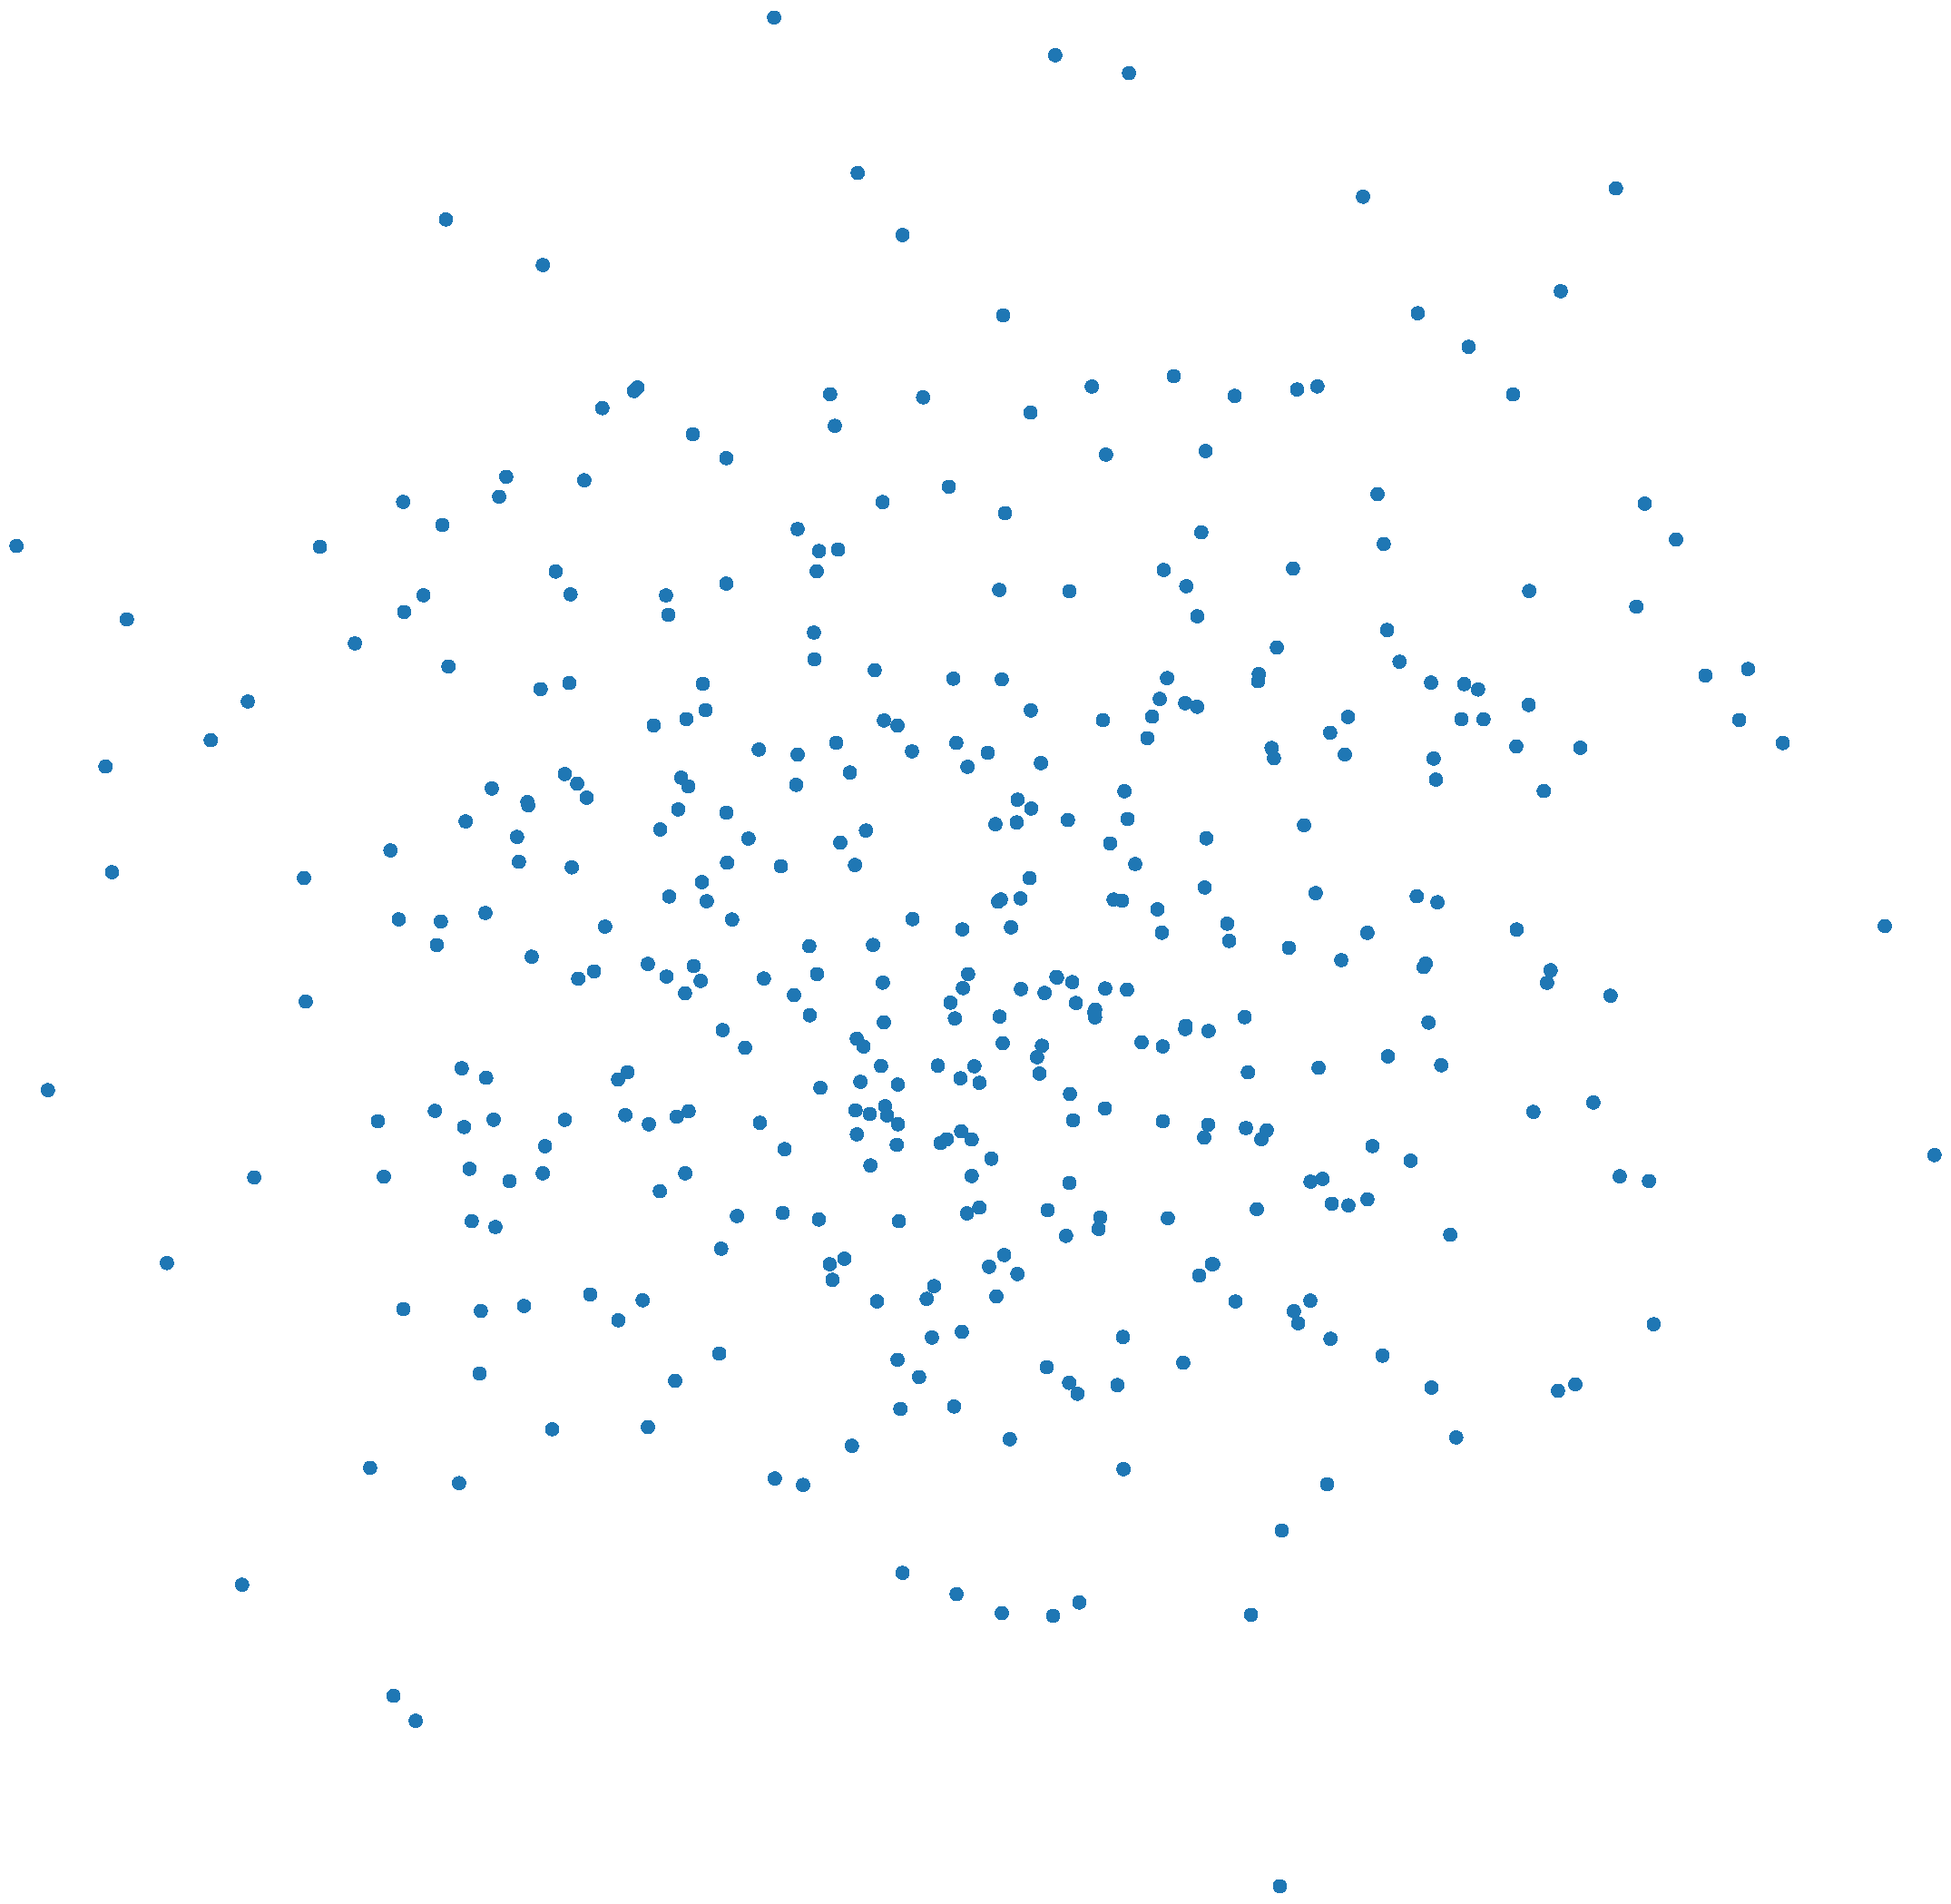
\includegraphics[width=.3\textwidth]{images/moon/zdist-crop.pdf}};
  \node[inner sep=0pt, right= 0.2cm of ffnn] (latentx) {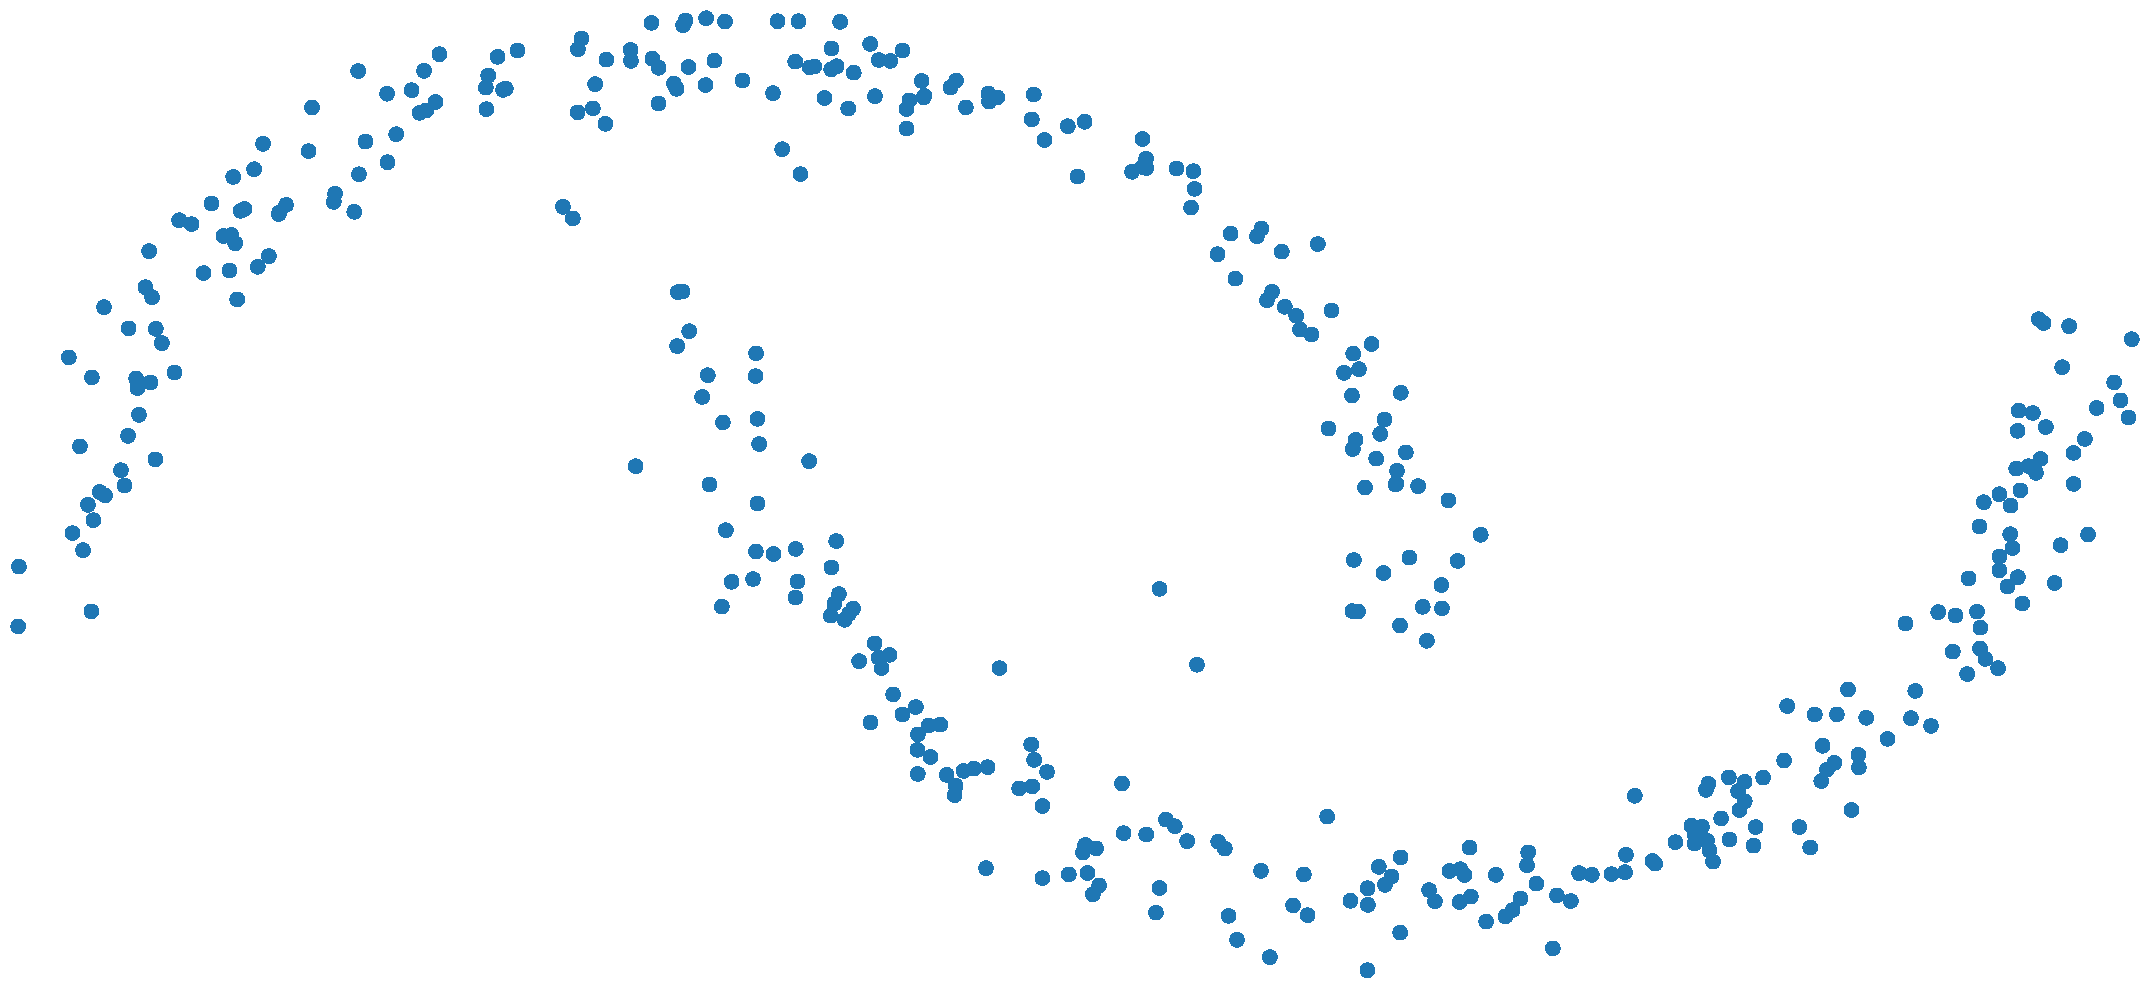
\includegraphics[width=.3\textwidth]{images/moon/xdist-crop.pdf}};
  
\end{scope}
%%% Local Variables:
%%% mode: latex
%%% TeX-master: "../ppgm_slide"
%%% End:

    \end{scope}
    \node [black, below=-0.05cm of illFlow] (changeveq) {
      \scriptsize
      \begin{minipage}{0.7\textwidth}
        When the $k$-th generator is selected, i.e., $s_k=1$ and $s_{k^{\prime}}=0$  for $k^{\prime}\neq k$, say $\tilde{\bm{x}} = \bm{x}|_{s_k=1}$. By following the \href{https://online.stat.psu.edu/stat414/lesson/23/23.1}{change of variable rule}
        \vskip -0.4cm
        \begin{equation*}
          \underbrace{p(\tilde{\bm{x}})|_{\tilde{\bm{x}} = \tilde{\bm{g}}(\bm{z})}}_{\text{Induced distribution}} =  \underbrace{p(\bm{z})}_{\text{\begin{tabular}{c}Assumed known distribution \\ easy to sample\end{tabular}}}\cdot \underbrace{\bigg| \mathrm{det}\left({\pd{\bm{z}}{\tilde{\bm{x}}}}\right)\bigg|}_{\text{\begin{tabular}{c}Computational load\\ depends on the mapping\end{tabular}}}.
        \end{equation*}
        \only<1>{
          \vskip -0.4cm
          A toy example:\\
        }
        \only<2>{
          \vskip -0.4cm
          Powering it with a $L$-layer neural network implementation:
        }
      \end{minipage}};
    \draw[green, ->, shorten >=5pt, shorten <=5pt] ($(gk.north)+(0,0cm)$) -- ($(gk.north)+(0,-0.8cm)$);
    \only<1>{
      \begin{scope}[scale=0.8, shift={($(changeveq.south)+(-2.5cm,-0.7cm)$)}]
        \node[black] at (2.5cm, 0) {\scriptsize
          Gaussian linear transform: $Z \sim \mathsf{N}\left( 0, 1  \right)$ $\xrightarrow{X=\sigma\cdot Z + \mu}$ $X \sim \mathsf{N}\left( \mu, \sigma  \right)$
        };
      \end{scope}
    }
    \only<2>{
      \begin{scope}[scale=0.8, shift={($(changeveq.south)+(-2.5cm,-0.7cm)$)}]
        \node (z) at (0,0) {};
        \node at ($(z)-(0.5,0)$){$\bm{z}=\bm{h}_0$};
        \node (xi1) at (1.5,0) {$\bm{h}_1$};
        \node (xi2) at (3,0) {};
        \node (xi3) at (4.5,0){};
        \node (x) at (6,0) {};
        \node at ($(x)+(0.5,0)$){$\bm{x} = \bm{h}_L$};
        \draw[->] ($(z) + (0.3,0.1)$) -- node[above]{$\tilde{\bm{g}}_1$} ($(xi1)+(-0.3,0.1)$); 
        \draw[->] ($(xi1)-(0.3,0.1)$) -- node[below]{$\tilde{\bm{f}}_1$}($(z) - (-0.3,0.1)$);
        \draw[->] ($(xi1) + (0.3,0.1)$) -- node[above]{$\tilde{\bm{g}}_2$} ($(xi2)+(-0.3,0.1)$); 
        \draw[->] ($(xi2)-(0.3,0.1)$) -- node[below]{$\tilde{\bm{f}}_2$}($(xi1) - (-0.3,0.1)$);
        \draw[->] ($(xi3) + (0.3,0.1)$) -- node[above]{$\tilde{\bm{g}}_L$} ($(x)+(-0.3,0.1)$); 
        \draw[->] ($(x)-(0.3,0.1)$) -- node[below]{$\tilde{\bm{f}}_L$}($(xi3) - (-0.3,0.1)$);
        \draw[dotted,line width = 0.3 mm] (xi2) -- (xi3);
      \end{scope}
    }
    %%%%%%%%%%%%%%%%%%%%%%%%%%%%%%%%%%%%%%%% 
    %% 4. one layer mapping of the flow
    %%%%%%%%%%%%%%%%%%%%%%%%%%%%%%%%%%%%%%%% 
    
    \begin{scope}[shift={($(dgm.south)+(0,-3.5cm)$)}, scale=0.3, every node/.append style={transform shape}, local bounding box=oneLayer, opacity=\bgopacity]
      % \tikzstyle{enode} = [thick, draw=blue, circle, inner sep = 3pt,
% align=center]
\tikzstyle{enode} = [thick, draw=black, circle, inner sep = 0, minimum size = 1cm,  align=center]
\tikzstyle{nnode} = [thick, rectangle, rounded corners = 2pt,minimum size = 0.4cm,draw,inner sep = 2pt]
\node[enode] (hal) at (-2,1) {$\bm{h}_{l,a}$};
\node[enode] (hbl) at (-2,-1) {$\bm{h}_{l,b}$};
\node[enode] (hal-1) at (2,1) {$\bm{h}_{l-1,a}$};
\node[enode] (hbl-1) at (2,-1) {$\bm{h}_{l-1,b}$};
\node[nnode] (times) at (-0.5,-1) {$\times$};
\node[nnode] (plus) at (0.5,-1) {$+$};
\node[nnode] (eq) at (0,1) {$=$};
\draw[->] (hal) -- node[fill=white] {$m_a$} (times);
\draw[->] (hal) -- node[fill=white] {$m_b$} (plus);
\draw[->] (hal) to (eq);

\draw[->] (eq) to (hal-1);
\draw[->] (hbl) to (times);
\draw[->] (times) to (plus);
\draw[->] (plus) to (hbl-1);
% \draw[draw=black] (-0.5,-0.5) rectangle ++(1,2);

%%% Local Variables:
%%% mode: latex
%%% TeX-master: "../ppgm_slide"
%%% End:

    \end{scope}
    \draw[dashed, ->, shorten >=5pt, shorten <=5pt, opacity=\bgopacity] ($(oneLayer.east)+(1.5cm,0cm)$) -- ($(oneLayer.east)+(0.1cm,0)$);
    
  \end{tikzpicture}
\end{frame}



\begin{frame}[label=current]{A High-level View of GenMM: Zoom into Layer}
  \begin{tikzpicture}
    \tikzstyle{enode} = [thick, draw=black, circle, align=center]
    \tikzstyle{cnode} = [thick, draw=black, circle, align=center, inner sep = 0.3pt]
    \tikzstyle{nnode} = [thick, rectangle, rounded corners = 2pt,minimum size = 0.8cm,draw,inner sep = 22pt]
    %%%%%%%%%%%%%%%%%%%%%%%%%%%%%%%%%%%%%%%% 
    %% 1. directed graphical model
    %%%%%%%%%%%%%%%%%%%%%%%%%%%%%%%%%%%%%%%% 
    \begin{scope}[scale=0.4, every node/.append style={transform shape}, local bounding box=dgm, opacity=0.3]
      \node[enode] (x) at (0,0){$\bm{x}$};

\node[enode, above=of x] (s) {$\bm{s}$};
\node[enode, left=of s] (z) {$\bm{z}$};
\node[enode, right=of s] (pi) {$\bm{\pi}$};
\node[cnode, right=of x] (phi) {$\{ \bm{\theta}_k \}$};
\node[nnode, fit=(x)(z)(s)] (box) {};

\draw[->] (z) to (x);
\draw[->] (s) to (x);
\draw[->] (pi) to (s);
\draw[->] (phi) to (x);

%%% Local Variables:
%%% mode: latex
%%% TeX-master: "../ppgm_slide"
%%% End:

    \end{scope}
    
    %%%%%%%%%%%%%%%%%%%%%%%%%%%%%%%%%%%%%%%% 
    %% 2. illustration of GenMM
    %%%%%%%%%%%%%%%%%%%%%%%%%%%%%%%%%%%%%%%% 
    \begin{scope}[scale=0.3, every node/.append style={transform shape}, shift={($(dgm.east)+(20cm,0)$)}, local bounding box=illsGenMM, opacity=\bgopacity]
      
% \tikzstyle{enode} = [thick, draw=blue, circle, inner sep = 3pt,
% align=center]
\tikzstyle{enode} = [thick, draw=black, ellipse, inner sep = 2pt,  align=center]
\tikzstyle{nnode} = [thick, rectangle, rounded corners = 2pt,minimum size = 0.8cm,draw,inner sep = 2pt]
\node[enode,label={below:{\tiny Shared latent source}}] (z) at (0,0) {$\bm{z}\sim p(\bm{z})$};
\node[enode, label={below:{\tiny Induced distribution}}] (x) at (5.5,0){$\bm{x}\sim p(\bm{x}; \bm{\Phi})$};
% \node at (5.2,-1) {$p(\bm{x};\bm{\Phi}) = \textstyle\sum_{k=1}^K \pi_k  p_k(\bm{x})$};
\node[nnode] (g1) at (2.6,1.8) {$\bm{g}_1$};
\node[nnode] (g2) at (2.6,0.5) {$\bm{g}_2$};
\node[nnode] (gk) at (2.6,-1.8) {$\bm{g}_K$};
\draw[dotted,line width=2pt] (2.6,-0.3) -- (2.6,-1.2);
\draw[->] (z) [in= 180, out =0] to (g1);
\draw[->] (z) [in= 180, out =0] to (g2);
\draw[->] (z) [in= 180, out =0] to (gk);
\filldraw[->] (3.7, 0.5)circle (2pt) -- node[above=0.2](switch){$\bm{s}\sim \bm{\pi}$} (x);
\node[above= 0.2 of switch.east] {\tiny \begin{tabular}{c}Categorical variable\\ as generator switch\end{tabular}};
% \draw[->] (3,-0.8) -- (3.5, -0.8);
\draw[->] (g1) -- (3.5,1.8);
\draw[->] (g2) -- (3.5, 0.5);
\draw[->] (gk) -- (3.5, -1.8);
\begin{scope}[on background layer, every node/.append style={transform shape}]
\node [rounded corners = 2pt, inner sep=4pt, fill=blue!30,fit=(g1)(g2)(gk), label={[label distance=0.3cm]-60:{\tiny Mixture of generators}}] {};
\end{scope}
%%% Local Variables:
%%% mode: latex
%%% TeX-master: "../ppgm_slide"
%%% End:

    \end{scope}
    \draw[dashed, ->, shorten >=5pt, shorten <=5pt, opacity=\bgopacity] (dgm) --node [text width=2cm, black, midway,above]{} (illsGenMM);
    
    %%%%%%%%%%%%%%%%%%%%%%%%%%%%%%%%%%%%%%%% 
    %% 3. illustration of flow
    %%%%%%%%%%%%%%%%%%%%%%%%%%%%%%%%%%%%%%%% 

    \begin{scope}[shift={($(illsGenMM.south)+(-0.5cm,0cm)$)}, scale=0.5, local bounding box=illFlow, opacity=\bgopacity]
      \def\layersep{1.5cm}
\begin{scope}[shorten >=1pt,->,draw=black!50, node distance=\layersep, scale=0.6, every node/.append style={transform shape},transform shape, local bounding box=ffnn]
  \tikzstyle{every pin edge}=[<-,shorten <=1pt]
  \tikzstyle{neuron}=[circle,fill=black!50,minimum size=17pt,inner sep=0pt]
  \tikzstyle{input neuron}=[neuron, fill=green!80];
  \tikzstyle{output neuron}=[neuron, fill=red!80];
  \tikzstyle{hidden neuron}=[neuron, fill=blue!80];
  \tikzstyle{annot} = [text width=4em, text centered]

  % Draw the input layer nodes
  \foreach \name / \y in {1,...,4}
  % This is the same as writing \foreach \name / \y in {1/1,2/2,3/3,4/4}
  % \node[input neuron, pin=left:Input \#\y] (I-\name) at (0,-\y) {};
  \node[input neuron, pin=left:{}] (I-\name) at (0,-\y) {};


  % Draw the hidden layer nodes
  \foreach \name / \y in {1,...,4}
  \path[yshift=0.0cm] node[hidden neuron] (H-\name) at (\layersep,-\y cm) {};

  % Draw the output layer node
  \foreach \name / \y in {1,...,4}
  \node[output neuron,pin={[pin edge={->}]right:{}}] (O-\name) at (2*\layersep, -\y cm) {};

  % Connect every node in the input layer with every node in the
  % hidden layer.
  \foreach \source in {1,...,4}
  \foreach \dest in {1,...,4}
  \draw[-{Stealth[scale=0.5]}] (I-\source) edge (H-\dest);

  % Connect every node in the hidden layer with the output layer
  \foreach \source in {1,...,4}
  \foreach \dest in {1,...,4}
  \draw[-{Stealth[scale=0.5]}] (H-\source) edge (O-\dest);

  % \foreach \source in {1,...,4}
  % \path (H-\source) edge (O);

  % Annotate the layers
  % \node[annot,above of=H-1, node distance=1cm] (hl) {Hidden layer};
  % \node[annot,left of=hl] {Input layer};
  % \node[annot,right of=hl] {Output layer};
  \node[inner sep=0pt, left= 0.2cm of ffnn] (latentz) {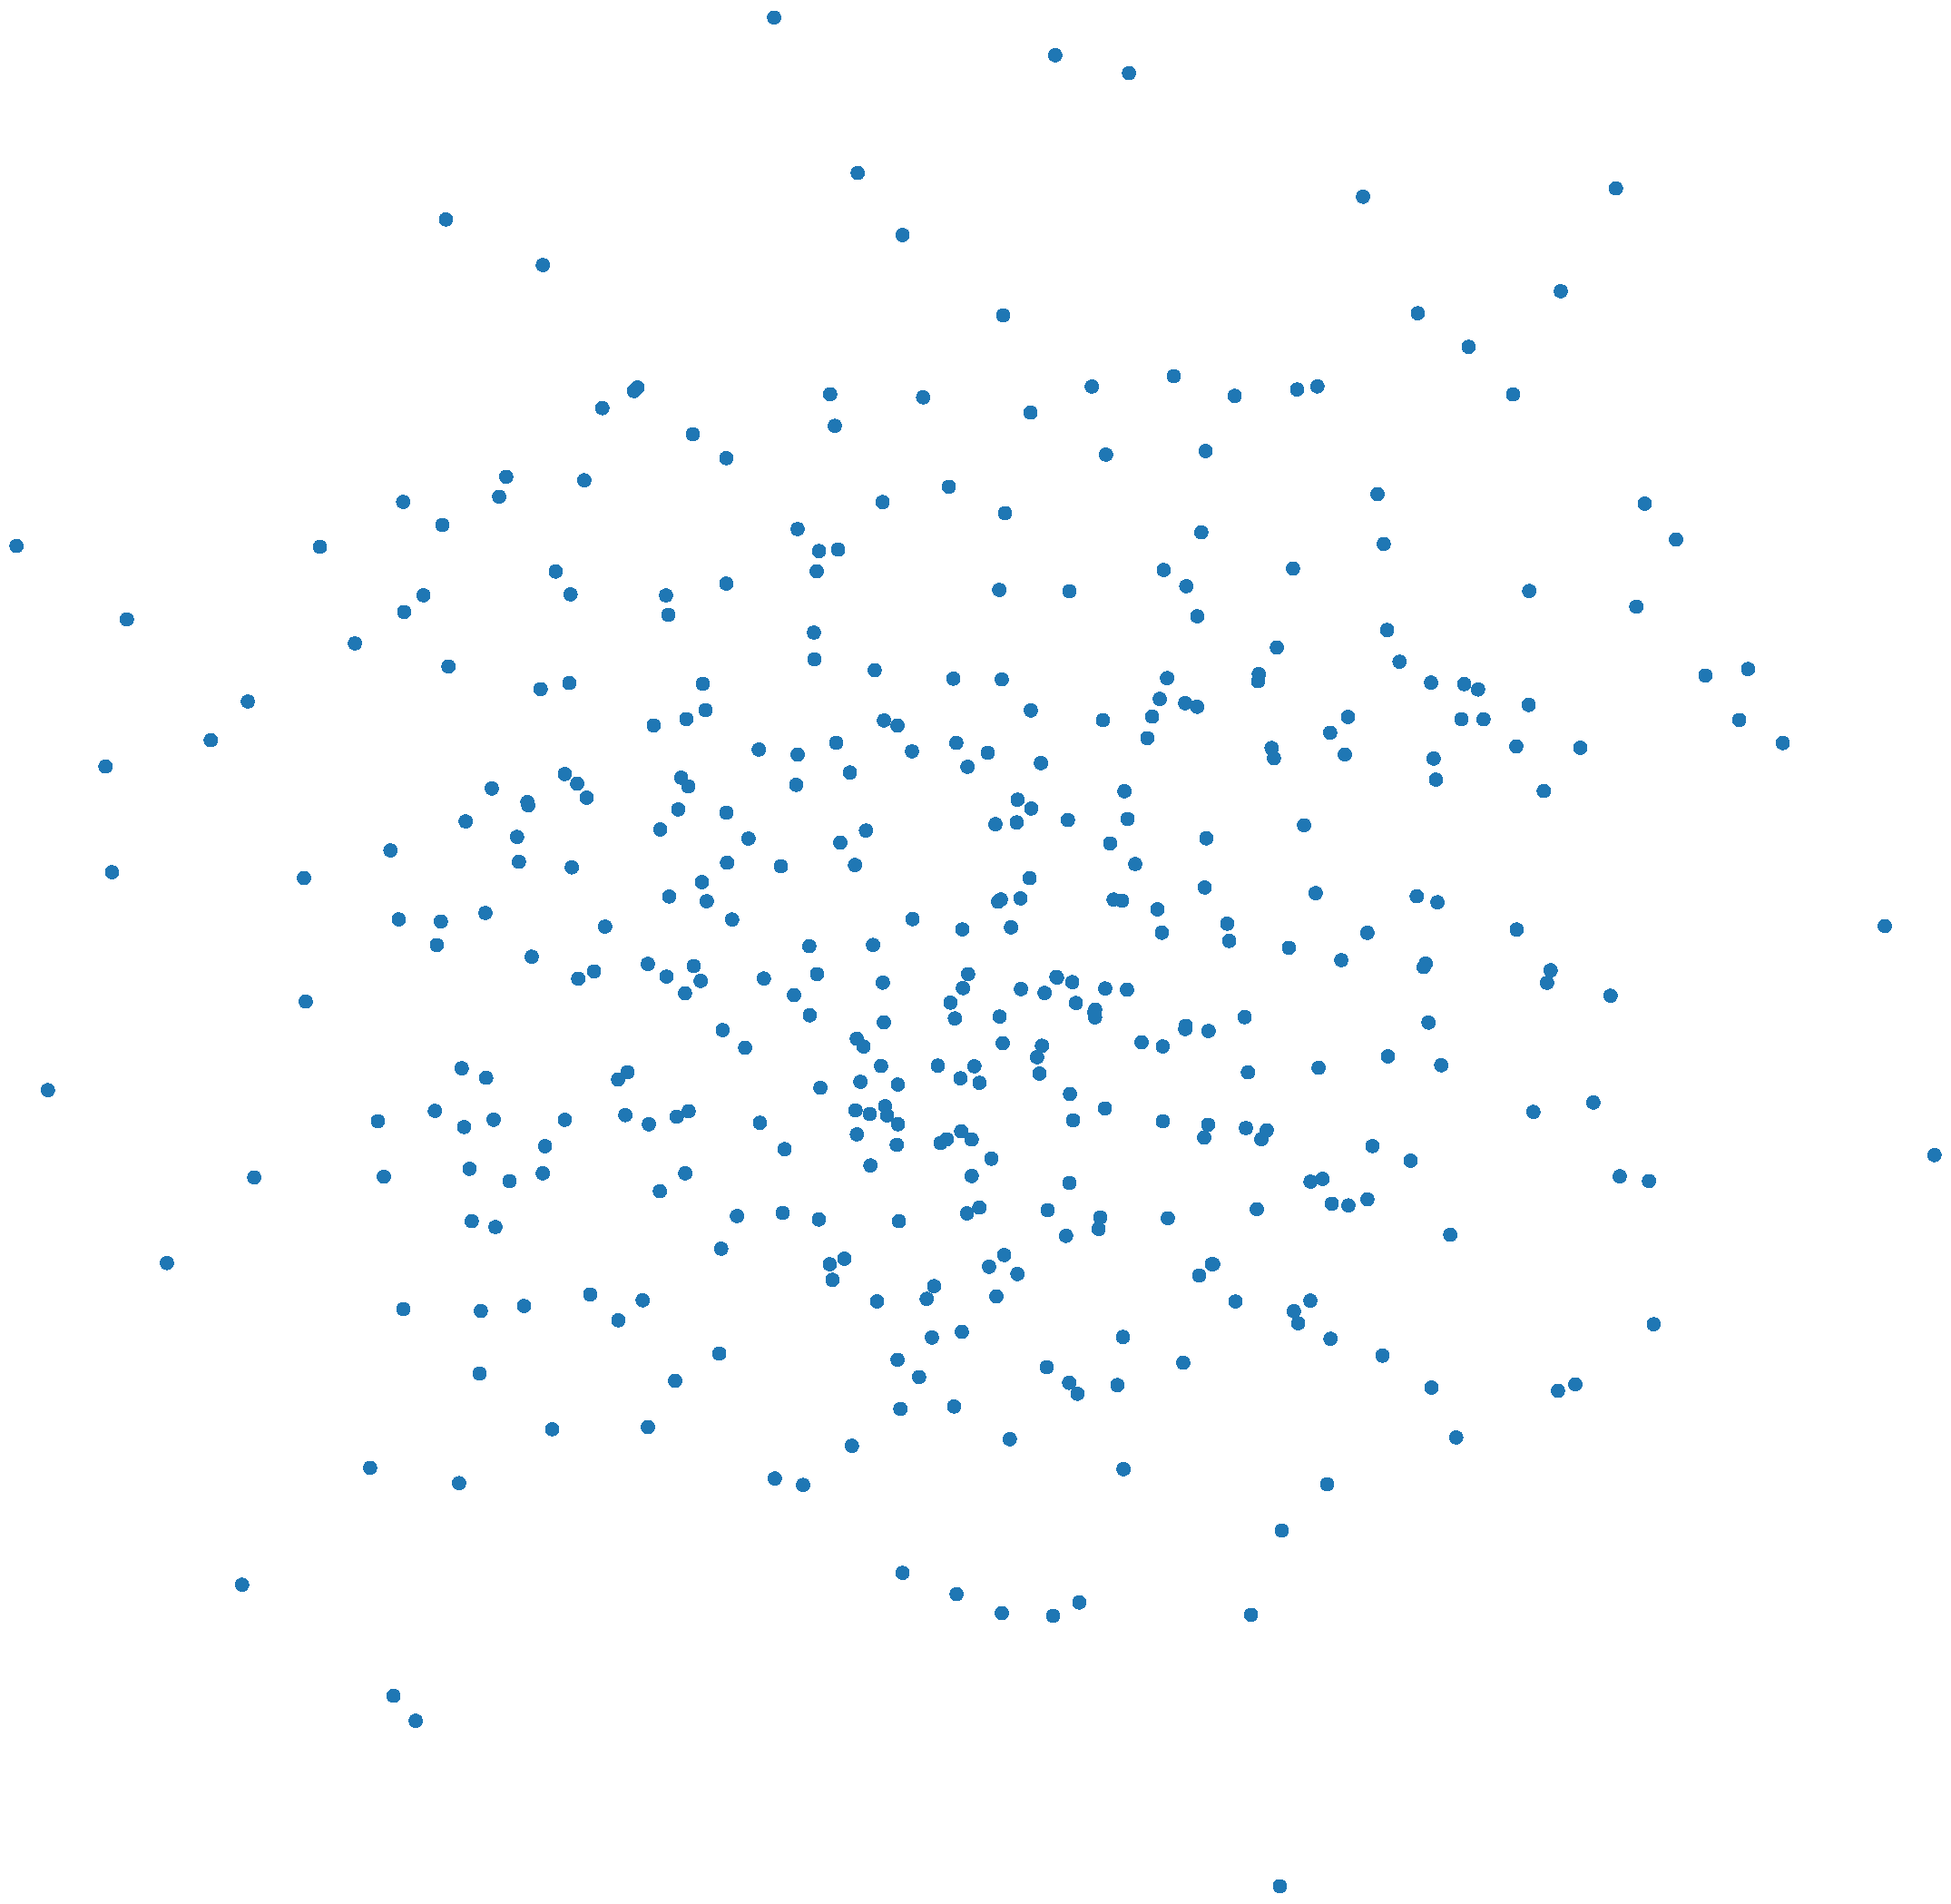
\includegraphics[width=.3\textwidth]{images/moon/zdist-crop.pdf}};
  \node[inner sep=0pt, right= 0.2cm of ffnn] (latentx) {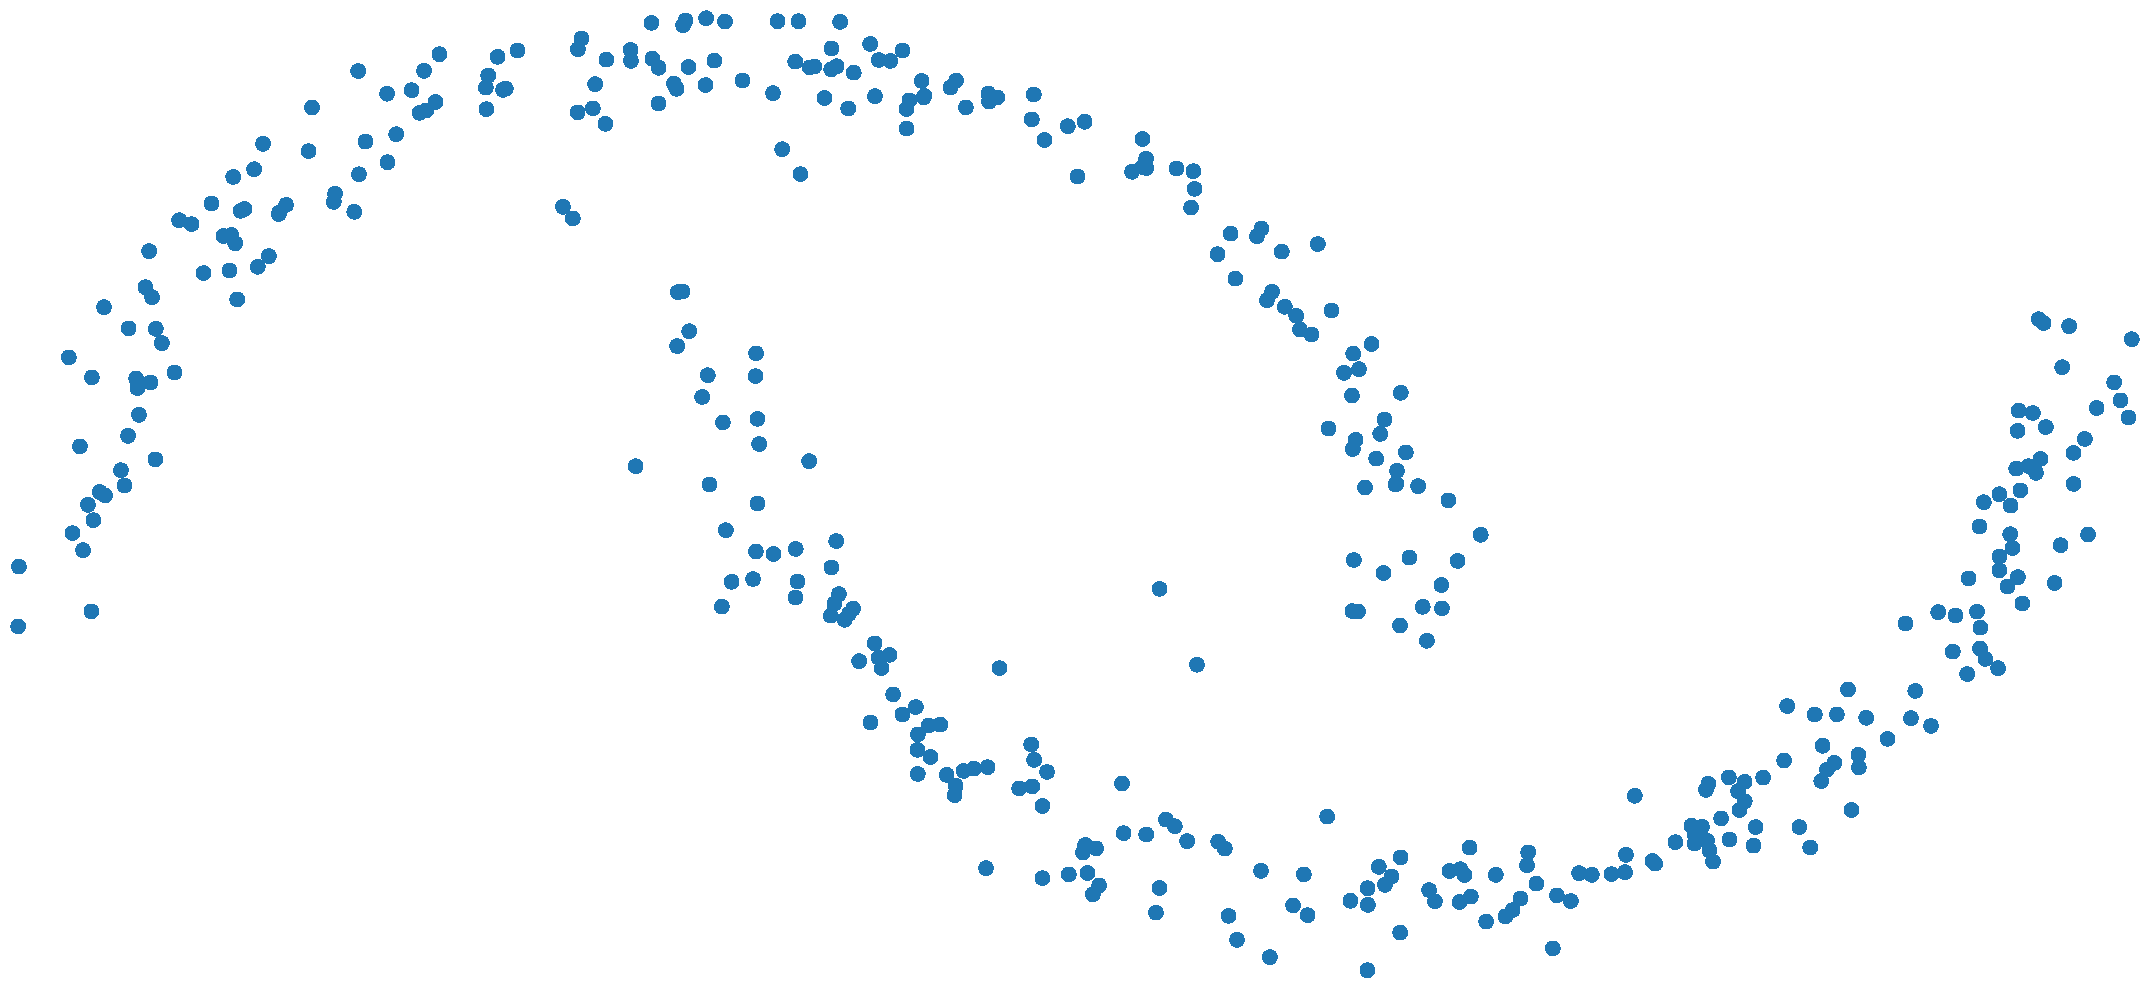
\includegraphics[width=.3\textwidth]{images/moon/xdist-crop.pdf}};
  
\end{scope}
%%% Local Variables:
%%% mode: latex
%%% TeX-master: "../ppgm_slide"
%%% End:

    \end{scope}
    \draw[dashed, ->, shorten >=5pt, shorten <=5pt, opacity=\bgopacity] ($(gk.north)+(0,0cm)$) -- ($(gk.north)+(0,-0.8cm)$);
    %%%%%%%%%%%%%%%%%%%%%%%%%%%%%%%%%%%%%%%% 
    %% 4. one layer mapping of the flow
    %%%%%%%%%%%%%%%%%%%%%%%%%%%%%%%%%%%%%%%% 
    
    \begin{scope}[shift={($(dgm.south)+(0,-1.5cm)$)}, scale=0.7, every node/.append style={transform shape}, local bounding box=oneLayer]
      % \tikzstyle{enode} = [thick, draw=blue, circle, inner sep = 3pt,
% align=center]
\tikzstyle{enode} = [thick, draw=black, circle, inner sep = 0, minimum size = 1cm,  align=center]
\tikzstyle{nnode} = [thick, rectangle, rounded corners = 2pt,minimum size = 0.4cm,draw,inner sep = 2pt]
\node[enode] (hal) at (-2,1) {$\bm{h}_{l,a}$};
\node[enode] (hbl) at (-2,-1) {$\bm{h}_{l,b}$};
\node[enode] (hal-1) at (2,1) {$\bm{h}_{l-1,a}$};
\node[enode] (hbl-1) at (2,-1) {$\bm{h}_{l-1,b}$};
\node[nnode] (times) at (-0.5,-1) {$\times$};
\node[nnode] (plus) at (0.5,-1) {$+$};
\node[nnode] (eq) at (0,1) {$=$};
\draw[->] (hal) -- node[fill=white] {$m_a$} (times);
\draw[->] (hal) -- node[fill=white] {$m_b$} (plus);
\draw[->] (hal) to (eq);

\draw[->] (eq) to (hal-1);
\draw[->] (hbl) to (times);
\draw[->] (times) to (plus);
\draw[->] (plus) to (hbl-1);
% \draw[draw=black] (-0.5,-0.5) rectangle ++(1,2);

%%% Local Variables:
%%% mode: latex
%%% TeX-master: "../ppgm_slide"
%%% End:

    \end{scope}
    \node [black, right=-0.5cm of oneLayer.east] {\scriptsize{Forward}};
    \node [black, below=1.3cm of oneLayer.west,anchor=west] (forwardmap) {
      \tiny
      \begin{minipage}{0.4\linewidth}
        \begin{equation*}
          \bm{h}_{l-1} =
          \begin{bmatrix}
            \bm{h}_{l-1,a}\\
            \bm{h}_{l-1,b}
          \end{bmatrix}
          =
          \begin{bmatrix}
            \bm{h}_{l,a}\\
            \bm{m}_a(\bm{h}_{l,a})\odot \bm{h}_{l,b} + \bm{m}_b(\bm{h}_{l,a})
          \end{bmatrix}
        \end{equation*}
      \end{minipage}
    };
    
    \begin{scope}[shift={($(oneLayer.south)+(0,-2.0cm)$)}, scale=0.7, every node/.append style={transform shape}, local bounding box=oneLayerInverse]
      % \tikzstyle{enode} = [thick, draw=blue, circle, inner sep = 3pt,
% align=center]
\tikzstyle{enode} = [thick, draw=blue, circle, inner sep = 0, minimum size = 1cm,  align=center]
\tikzstyle{nnode} = [thick, rectangle, rounded corners = 2pt,minimum size = 0.4cm,draw,inner sep = 2pt]
\node[enode] (hal) at (-2,1) {$\bm{h}_{l,a}$};
\node[enode] (hbl) at (-2,-1) {$\bm{h}_{l,b}$};
\node[enode] (hal-1) at (2,1) {$\bm{h}_{l-1,a}$};
\node[enode] (hbl-1) at (2,-1) {$\bm{h}_{l-1,b}$};
\node[nnode] (times) at (-0.5,-1) {$\div$};
\node[nnode] (plus) at (0.5,-1) {$-$};
\node[nnode] (eq) at (0,1) {$=$};
\draw[->] (hal-1) -- node[fill=white] {$\bm{m}_a$} (times);
\draw[->] (hal-1) -- node[fill=white] {$\bm{m}_b$} (plus);
\draw[<-] (hal) to (eq);

\draw[<-] (eq) to (hal-1);
\draw[->] (hbl) to (times);
\draw[<-] (times) to (plus);
\draw[<-] (plus) to (hbl-1);
% \draw[draw=black] (-0.5,-0.5) rectangle ++(1,2);


%%% Local Variables:
%%% mode: latex
%%% TeX-master: "../ppgm_slide"
%%% End:

    \end{scope}
    \node [black, right=-0.5cm of oneLayerInverse.east] {\scriptsize{Inverse}};

    \node [black, below=1.3cm of oneLayerInverse.west,anchor=west] (backwardmap) {
      \tiny
      \begin{minipage}{0.4\linewidth}
        \begin{equation*}
          \bm{h}_{l} =
          \begin{bmatrix}
            \bm{h}_{l,a}\\
            \bm{h}_{l,b}
          \end{bmatrix}
          =
          \begin{bmatrix}
            \bm{h}_{l-1,a}\\
            \left(  \bm{h}_{l-1,b} - \bm{m}_b(\bm{h}_{l-1,a}) \right)\oslash \bm{m}_a(\bm{h}_{l-1,a}) 
          \end{bmatrix}
        \end{equation*}
      \end{minipage}
    };

    \node [black, right=-0.5cm of oneLayerInverse.east] {\scriptsize{Inverse}};

    \node [black, right=2.3cm of oneLayerInverse.east,anchor=west] (attrtext) {
      \scriptsize
      \begin{minipage}{0.5\linewidth}
        \begin{itemize}[label=\textbullet]
        \item $\odot$ denotes element-wise product, $\oslash$ denotes
          element-wise division
        \item Mapping $\bm{m}_a$, $\bm{m}_b$ can be as complex as possible and not necessary invertible
        \item Same computation complexity of forward and inverse mapping
        \item Triangular matix of Jacobian
        \end{itemize}
        Alternative arch. on market: Auto-regressive flow, Glow, ODE, etc.
      \end{minipage}
    };
    \draw[green, ->] ($(oneLayer.east)+(3.5cm,0cm)$) --node [text width=5cm, black, right,above, anchor=north west]{\tiny Pick up one layer to zoom in} ($(oneLayer.east)+(1.1cm,0)$);
    
  \end{tikzpicture}
\end{frame}

\begin{frame}[label=current]
  {Alternative Mixture and Remark}
  \centering
  \begin{tikzpicture}[scale=0.7, every node/.append style={transform shape}]
    \tikzstyle{enode} = [thick, draw=black, ellipse, inner sep = 1pt,  align=center]
    \tikzstyle{nnode} = [thick, rectangle, rounded corners = 2pt,minimum size = 0.8cm,draw,inner sep = 2pt]
    \node[enode] (z1) at (0,1.8) {$\bm{z}\sim p_1(\bm{z})$};
    \node[enode] (z2) at (0,0.5){$\bm{z}\sim p_{2}(\bm{z})$};
    \node[enode] (zK) at (0,-1.8) {$\bm{z}\sim p_{K}(\bm{z})$}; 
    \node[enode, label={[label distance=0.3cm]-90:Induced Distribution}] (x) at (5.5,0){$\bm{x}\sim p(\bm{x};\ubar{\bm{\Phi}})$};
    
    \node[nnode, label={[label distance=0.5cm]-90:Share Generator}] (g) at (3.2,0) {$\bm{g}$};
    \draw[dotted,line width=2pt] (0,-0.3) -- (0,-1.2);
    \filldraw[->] (1.8, 0.5)circle (2pt) -- node[above=0.2]{$\bm{s}\sim \bm{\pi}$} (g) ;
    \draw[->] (z1) -- (1.6, 1.8);
    \draw[->] (z2) -- (1.6, 0.5);
    \draw[->] (zK) -- (1.6, -1.8);
    \begin{scope}[on background layer]
      \node[rounded corners = 4pt, rectangle, inner sep = 20pt,  align=center, fit=(z1)(z2)(zK), label=below:{Multiple Latent Sources}, fill=blue!30] (latSource) {};
    \end{scope}
    \draw[->] (g) to (x);
  \end{tikzpicture}
  
  \begin{block}{Remark On GenMM/GenHMM}
    \begin{itemize}[label=\textbullet]
    \item Free dimension for flexibility: number of mixture + complexity of functional form of neural networks
    \item Compatible with statistic methods and neural network techniques (error back-propagation, optimizer)
    \item Embed batch-gradient descent into M-step
    \item Lack of closed-form update rule and generator changes at each gradient step. We tackle by maintaining old and new generators in EM steps
    \end{itemize}
    
  \end{block}
\end{frame}


\begin{frame}[label=current]{Semantic Scores and Examples}
  \graphicspath{{/home/dong/Documents/phd_research/phdthesis/source/chapter6/}}
  \begin{figure}
    \captionsetup[subfigure]{justification=centering}
    \centering
    \begin{subfigure}{.24\textwidth}
      \centering
      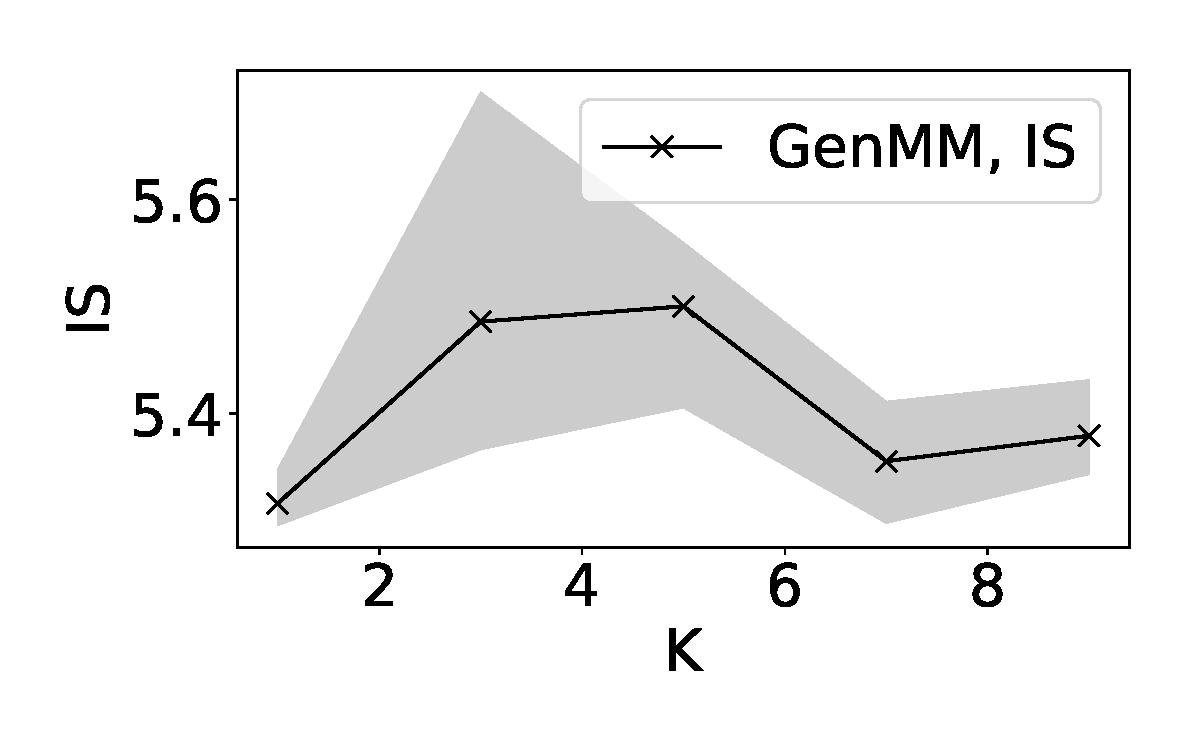
\includegraphics[width=1\linewidth]{images/mnist/scores/std1EMGM-NM/EMGM-NM-IS-K.pdf}
      % \caption{IS score}
      % \label{fig-nm-isk}
    \end{subfigure}
    \vspace{-2pt}
    \begin{subfigure}{.24\textwidth}
      \centering
      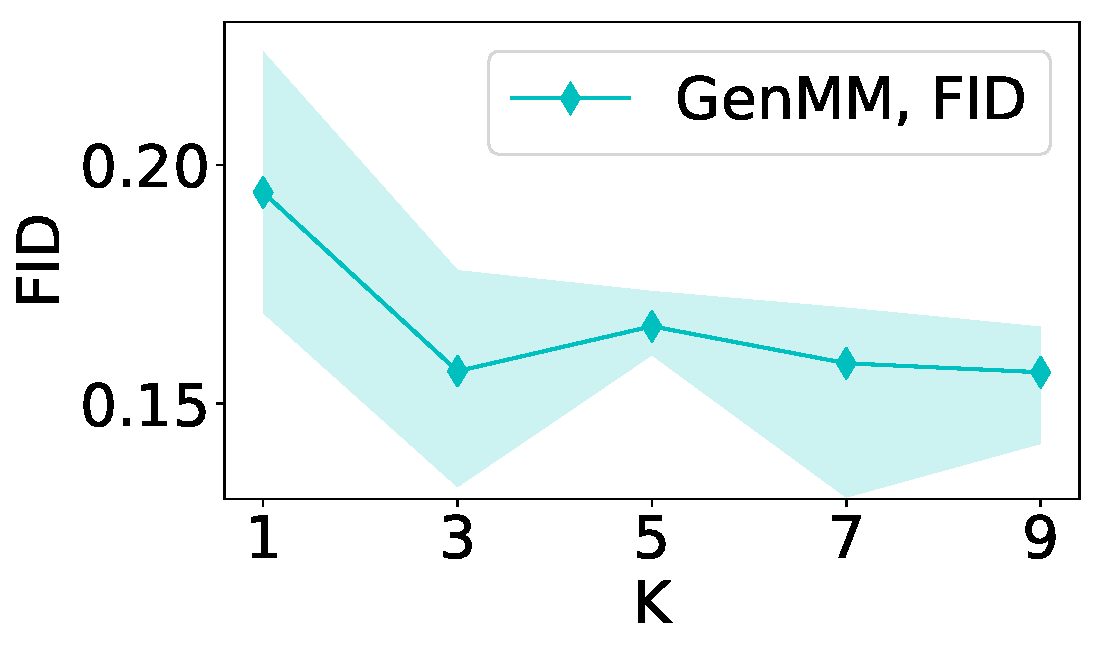
\includegraphics[width=1\linewidth]{images/mnist/scores/std1EMGM-NM/EMGM-NM-FID-K.pdf}
      % \caption{FID score}
      % \label{fig-nm-fidk}
    \end{subfigure}
    \centering
    \begin{subfigure}{.24\textwidth}
      \centering
      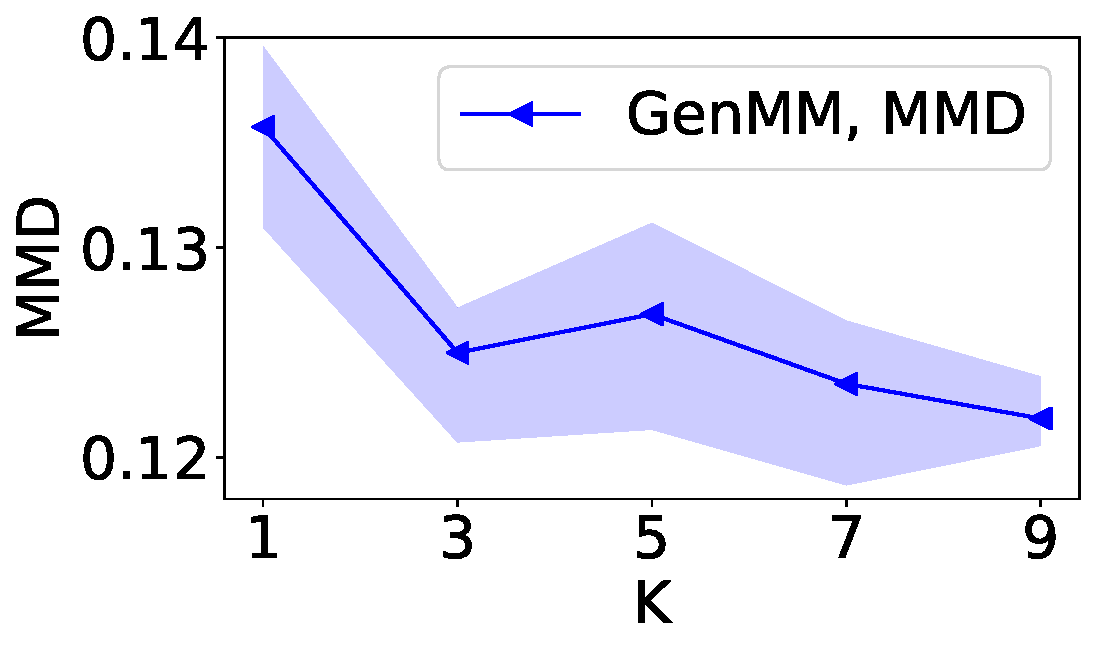
\includegraphics[width=1\linewidth]{images/mnist/scores/std1EMGM-NM/EMGM-NM-MMD-K.pdf}
      % \caption{MMD score}
      % \label{fig-nm-mmdk}
    \end{subfigure}
    \centering
    \begin{subfigure}{0.24\textwidth}
      \centering
      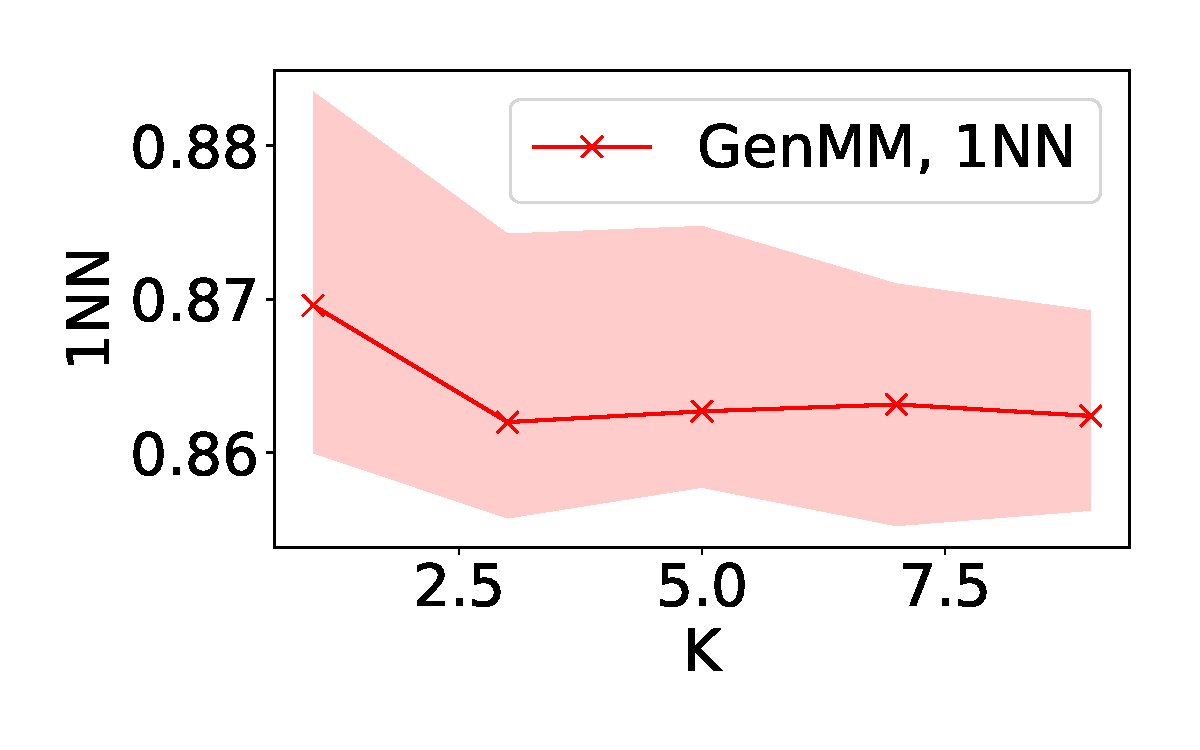
\includegraphics[width=1\linewidth]{images/mnist/scores/std1EMGM-NM/EMGM-NM-1NN-K.pdf}
      % \caption{1NN score}
      % \label{fig-nm-1nnk}
    \end{subfigure}
    \centering
    \begin{subfigure}{.24\textwidth}
      \centering
      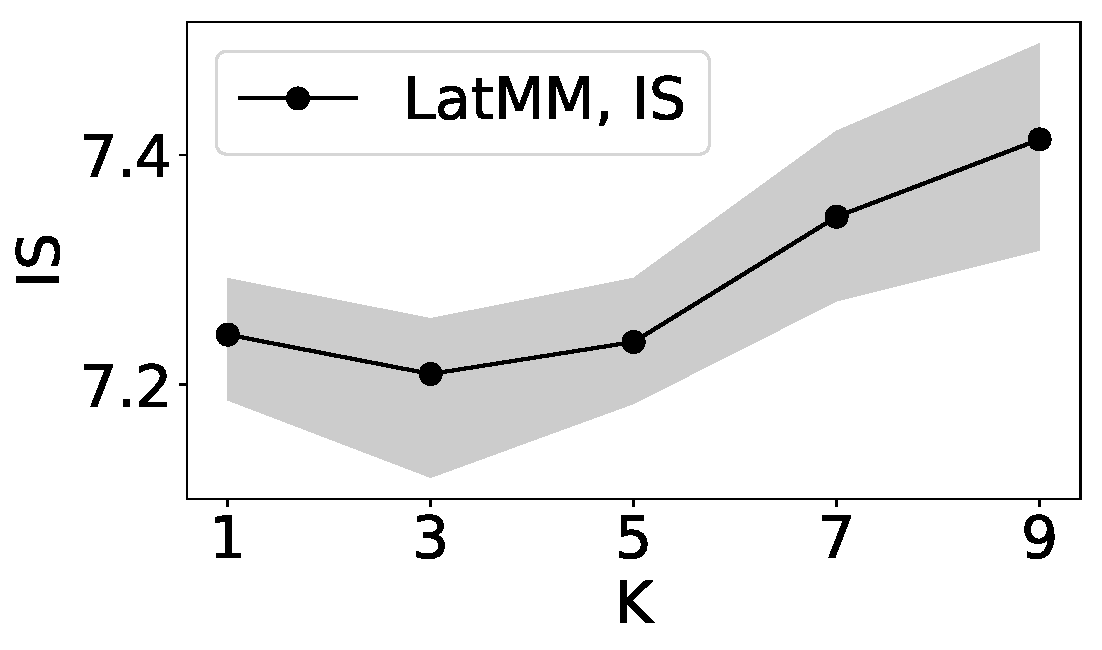
\includegraphics[width=1\linewidth]{images/mnist/scores/std1EMGM-SM/EMGM-SM-IS-K.pdf}
      % \caption{IS score}
      % \label{fig-sm-is}
    \end{subfigure}
    \centering
    \begin{subfigure}{.24\textwidth}
      \centering
      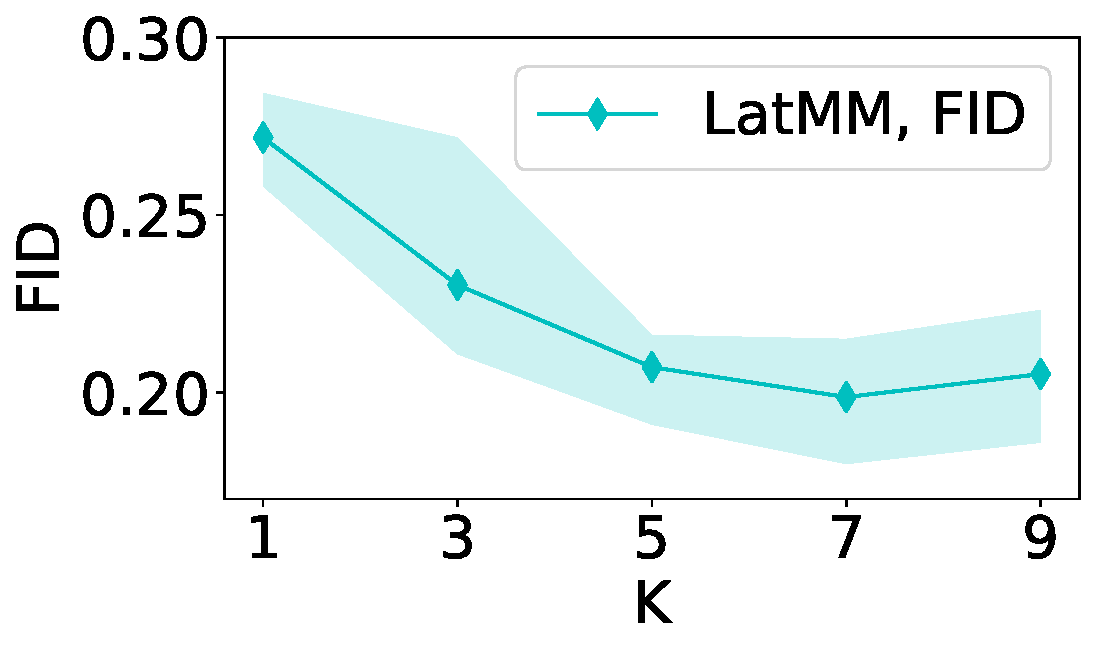
\includegraphics[width=1\linewidth]{images/mnist/scores/std1EMGM-SM/EMGM-SM-FID-K.pdf}
      % \caption{FID score}
      % \label{fig-sm-fid}
    \end{subfigure}
    \centering
    \begin{subfigure}{.24\textwidth}
      \centering
      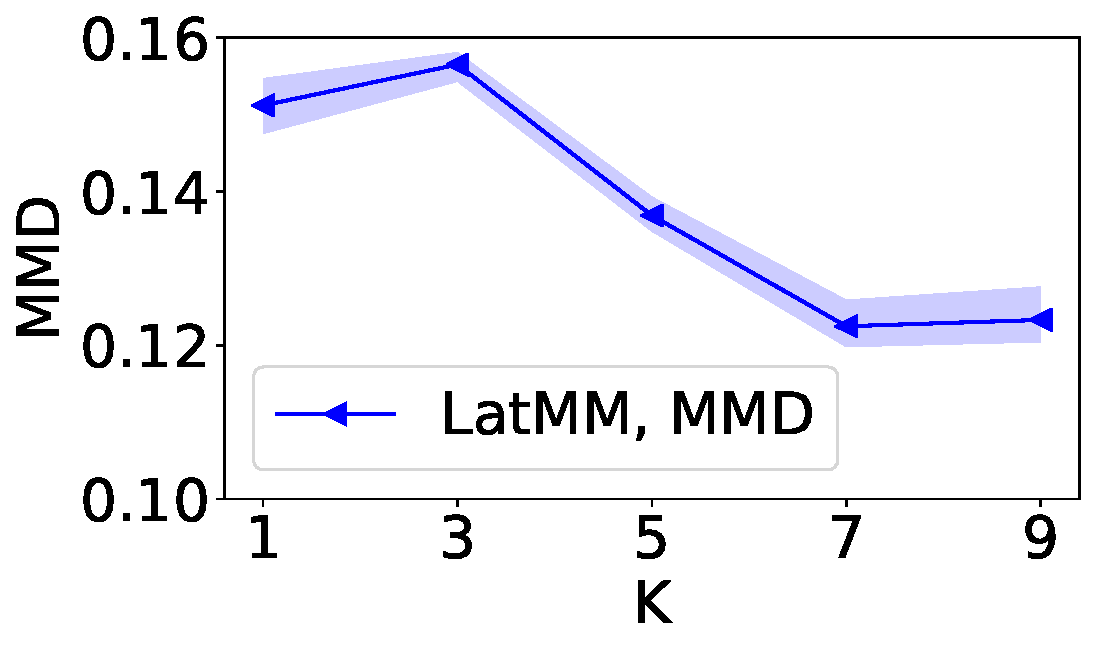
\includegraphics[width=1\linewidth]{images/mnist/scores/std1EMGM-SM/EMGM-SM-MMD-K.pdf}
      % \caption{MMD score}
      % \label{fig-sm-mmd}
    \end{subfigure}
    \begin{subfigure}{0.24\textwidth}
      \centering
      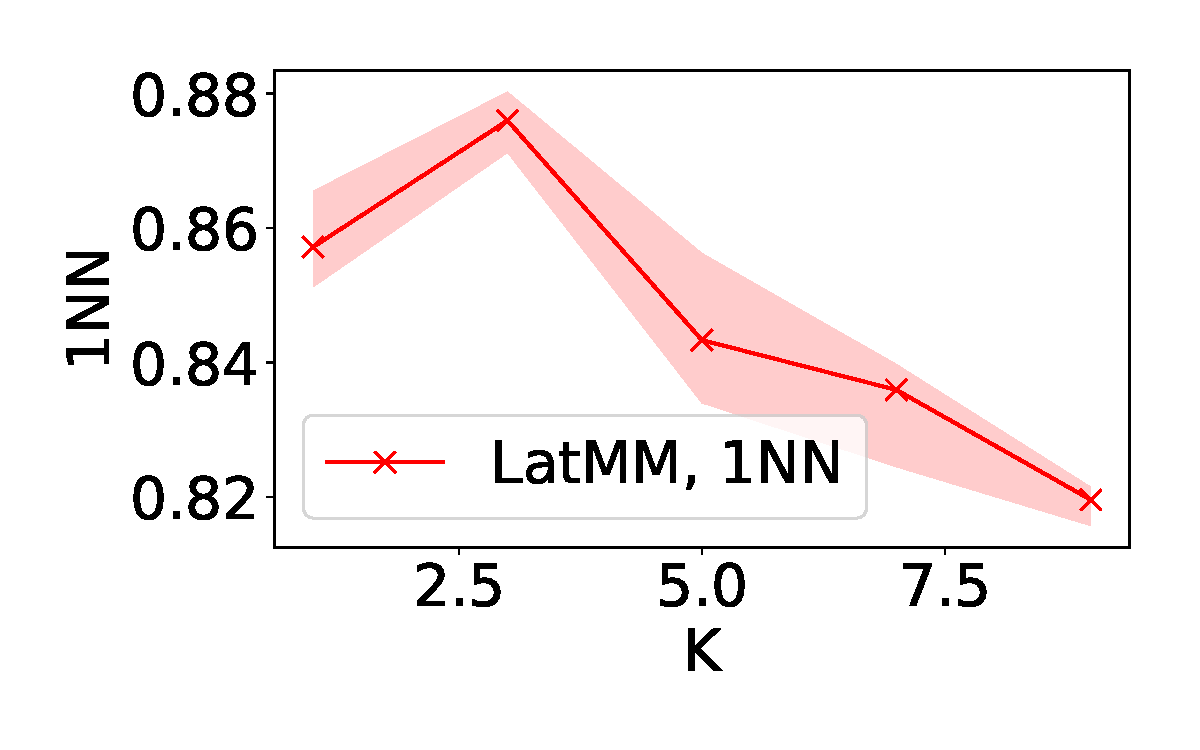
\includegraphics[width=1.\linewidth]{images/mnist/scores/std1EMGM-SM/EMGM-SM-1NN-K.pdf}
      % \caption{1NN score}
      % \label{fig-sm-1nn}
    \end{subfigure}
  \end{figure}
  \only<1>{
    IS, FID, MMD and 1NN of GenMM and LatMM for MNIST dataset.
    \begin{itemize}
    \item[-]{IS: Inseption Score}
    \item[-]{FID: Frechet Inception Distance}
    \item[-]{MMD: Maximum Mean Discrepancy}
    \item[-]{1NN: 1-Nearest Neighbor}
    \end{itemize}
    \vfill
  }
  \only<2>{
    \vskip -0.7cm
    \begin{columns}
      \column{0.5\textwidth}
      \centering
      \begin{figure}[!t]
        \captionsetup[subfigure]{justification=centering}
        \centering
        \begin{subfigure}[b]{0.45\textwidth}
          \centering
          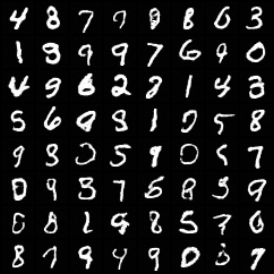
\includegraphics[width=1\linewidth]{images/mnist/samples/genMNIST_GenMM_K7_std089.png}

        \end{subfigure}
        \hspace{5pt}
        \begin{subfigure}[b]{0.45\textwidth}
          \centering
          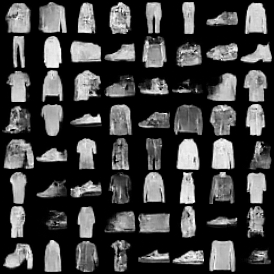
\includegraphics[width=1\linewidth]{images/fashion-mnist/samples/gen_s7_std1.png}
          %     \caption{Generated samples. (LatMM, K=7)}
        \end{subfigure}
        \vspace{-0.2cm}
      \end{figure}
      Generated samples by GenMM and LatMM.

      
      \column{0.5\textwidth}
      \centering
      \begin{figure}
        \centering
        \captionsetup[subfigure]{justification=centering}
        \begin{subfigure}[b]{0.43\textwidth}
          \centering
          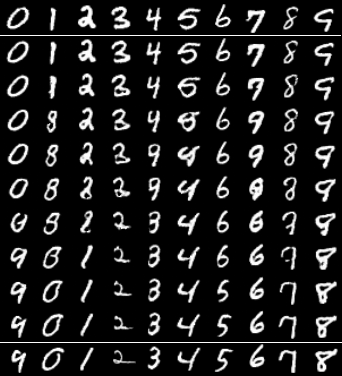
\includegraphics[width=1\linewidth]{images/mnist/interpolation/interpoMNIST_heter_LatMM_K9_sample_grid.png}
          %     \caption{Interpolation by LatMM, K=9.}\label{fig-interpo-latmm2}
        \end{subfigure}
        \hspace{5pt}
        \begin{subfigure}[b]{0.43\textwidth}
          \centering
          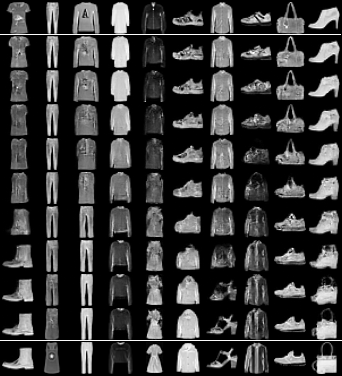
\includegraphics[width=1\linewidth]{images/fashion-mnist/interpolation/interpoFashion_heter_LatMM_K9_grid.png}
          %     \caption{Interpolation by LatMM, K=9.}\label{fig-interpo-latmm3}
        \end{subfigure}
        \vspace{-0.2cm}
      \end{figure}
      Interpolation in latent space
  \end{columns}
}
\end{frame}

\begin{frame}[label=current]{Application to Classification Tasks}
  Application to classification with maximum likelihood. Test Accuracy Table of GenMM for Classification Task
  \begin{table}
    \centering
    \begin{tabular}{lccccccc} \toprule
      {Dataset} &  K=1 &  K=2 &  K=3 &  K=4 & K=10 & K=20 & State Of Art \\ \midrule
      Letter & 0.9459 &  0.9513 & 0.9578  & 0.9581 & 0.9657 & \textbf{0.9674} & {0.9582}  \\ \midrule
      Satimage & 0.8900 & 0.8975 & 0.9045 & 0.9085 & 0.9105 & \textbf{0.9160} & 0.9090    \\ \midrule
      Norb & 0.9184 & 0.9257 & 0.9406 & 0.9459 & 0.9538 & \textbf{0.9542} & 0.8920   \\
      \bottomrule
    \end{tabular}

  \end{table}
\end{frame}

%%% Local Variables:
%%% mode: latex
%%% TeX-master: "../ppgm_slide"
%%% End:
